\documentclass[10pt,journal,compsoc]{IEEEtran}


% *** CITATION PACKAGES ***
%
\ifCLASSOPTIONcompsoc
  % IEEE Computer Society needs nocompress option
  % requires cite.sty v4.0 or later (November 2003)
  \usepackage[nocompress]{cite}
\else
  % normal IEEE
  \usepackage{cite}
\fi

\usepackage[numbers]{natbib}

\usepackage{cite}
\usepackage{amsmath,amssymb,amsfonts}
\usepackage{algorithmic}
\usepackage{graphicx}
\usepackage{textcomp}
\usepackage{xcolor}
\usepackage[framemethod=TikZ]{mdframed}
\usepackage{multirow}
\usepackage{array}
\usepackage{lipsum}
% \usepackage{subfigure}
\usepackage{caption}
\usepackage{subcaption}
\usepackage{hyperref}
\usepackage{longtable}


\newcommand{\specialcell}[2][c]{%
  \begin{tabular}[#1]{@{}c@{}}#2\end{tabular}}

\usepackage{xspace}
\newcommand{\instance}{{\em CTO}\xspace}
\newcommand{\inconsistent}{{\em IoPV}\xspace}

\newcommand{\ian}[1]{\textcolor{red}{{\it [Ian says: #1]}}}
\newcommand{\bram}[1]{\textcolor{orange}{{\it [Bram says: #1]}}}
\newcommand{\heng}[1]{\textcolor{blue}{{\it [Heng says: #1]}}}
\newcommand{\med}[1]{\textcolor{cyan}{{\it [Mohammed says: #1]}}}
\newcommand{\jinfu}[1]{\textcolor{purple}{{\it [Jinfu says: #1]}}}
% \newcommand{\heng}[1]{\textcolor{green}{{\it [Heng says: #1]}}}

\def\BibTeX{{\rm B\kern-.05em{\sc i\kern-.025em b}\kern-.08em
    T\kern-.1667em\lower.7ex\hbox{E}\kern-.125emX}}
    
    
\usepackage[most]{tcolorbox}

\hypersetup{
  colorlinks,
  citecolor=blue,
  linkcolor=red,
  urlcolor=purple}

\definecolor{custom-gray}{cmyk}{0, 0, 0, 0.7, 1.00}
\newtcbtheorem[no counter]{Summary}{\hskip-0.97em}{enhanced,drop shadow={black!50!white},
  coltitle=white,
  top=0.1in,
  attach boxed title to top left=
  {xshift=1em,yshift=-\tcboxedtitleheight/2},
  boxed title style={size=small,colback=custom-gray}
}{summary}

\newcommand{\PQI}{Are \inconsistent issues common in the studied systems? }
\newcommand{\PQII}{How difficult is it to manually identify \inconsistent issues?}

\newcommand{\RQI}{What is the impact of configuration on performance regression?}
\newcommand{\RQII}{Can we accurately learn \inconsistent issues in the studied systems? }
\newcommand{\RQIII}{What are the most important metrics for predicting \inconsistent issues? }


\usepackage{booktabs} % For formal tables

\usepackage{flushend} % makes the last page balanced

\usepackage{balance}

\usepackage{enumitem}
\newlist{steps}{enumerate}{1}
\setlist[steps, 1]{label = Step \arabic*:}

% code listing
\usepackage{listings}
%\usepackage{xcolor}
\definecolor{dkgreen}{rgb}{0,0.6,0}
\definecolor{gray}{rgb}{0.5,0.5,0.5}
\definecolor{mauve}{rgb}{0.58,0,0.82}
\lstset{frame=tb,
	language=Java,
	aboveskip=3mm,
	belowskip=3mm,
	showstringspaces=false,
	captionpos=b,
	columns=flexible,
	%columns=fullflexible
	%basicstyle={\small\ttfamily},
	basicstyle=\linespread{1.1}\footnotesize, 
	numbers=none,
	numberstyle=\tiny\color{gray},
	keywordstyle=\color{blue},
	commentstyle=\color{dkgreen},
	stringstyle=\color{mauve},
	breaklines=true,
	breakatwhitespace=true,
	tabsize=3,
	escapeinside={(*}{*)}
}
\lstdefinestyle{interfaces}{
	float=tp,
	floatplacement=tbp
}

\newcommand{\specialcell}[2][c]{%
	\begin{tabular}[#1]{@{}c@{}}#2\end{tabular}}
\newcommand{\specialleft}[2][l]{%
	\begin{tabular}[#1]{@{}l@{}}#2\end{tabular}}
\newcommand{\specialright}[2][r]{%
	\begin{tabular}[#1]{@{}r@{}}#2\end{tabular}}
	
\makeatletter
\newcommand\footnoteref[1]{\protected@xdef\@thefnmark{\ref{#1}}\@footnotemark}
\makeatother

\usepackage{url}
\usepackage[flushleft]{threeparttable}

    
\begin{document}

\begin{figure*}
	\centering
        \begin{subfigure}{0.19\textwidth}
                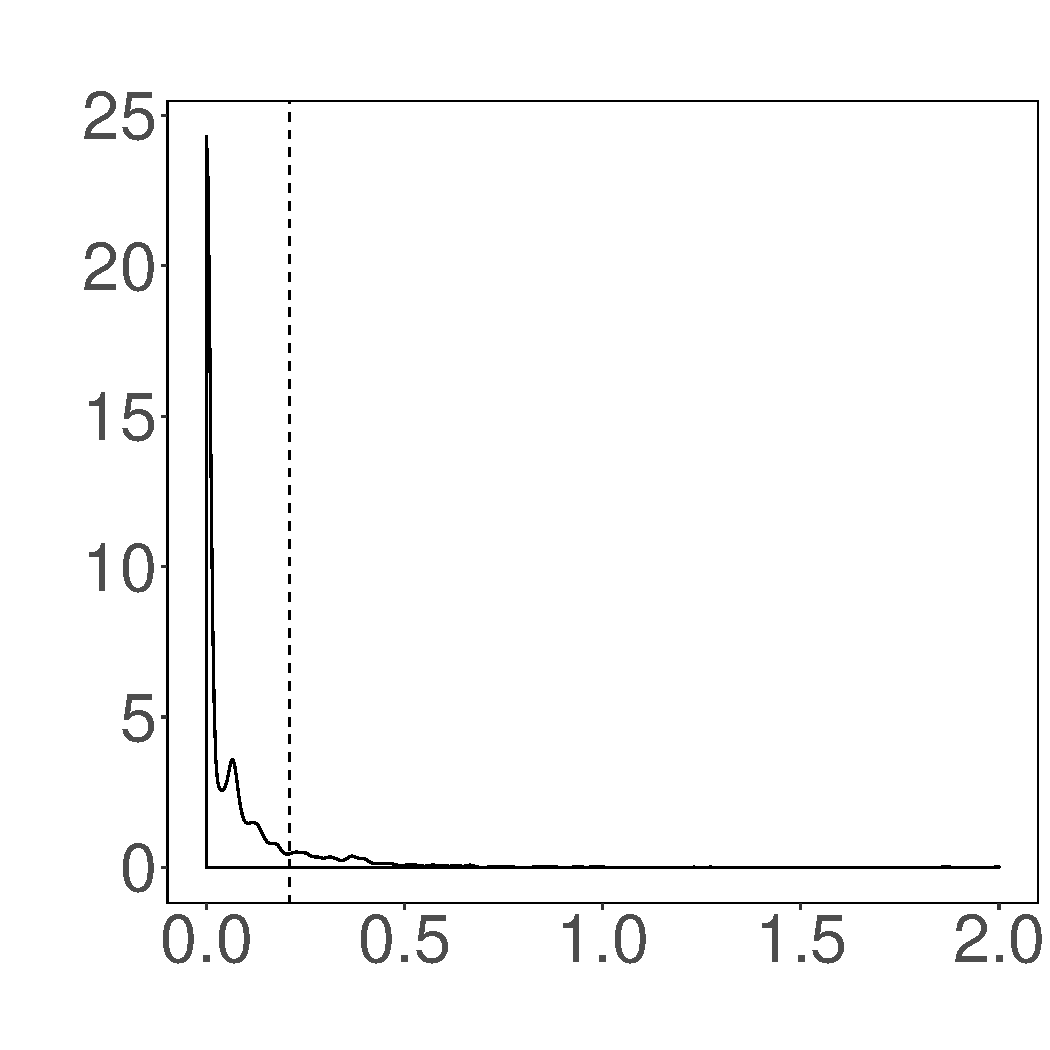
\includegraphics[width=\linewidth]{Figures/runtime-hadoop-cluster.pdf}
                \caption{Res. time}
        \end{subfigure}%
        \begin{subfigure}{0.19\textwidth}
                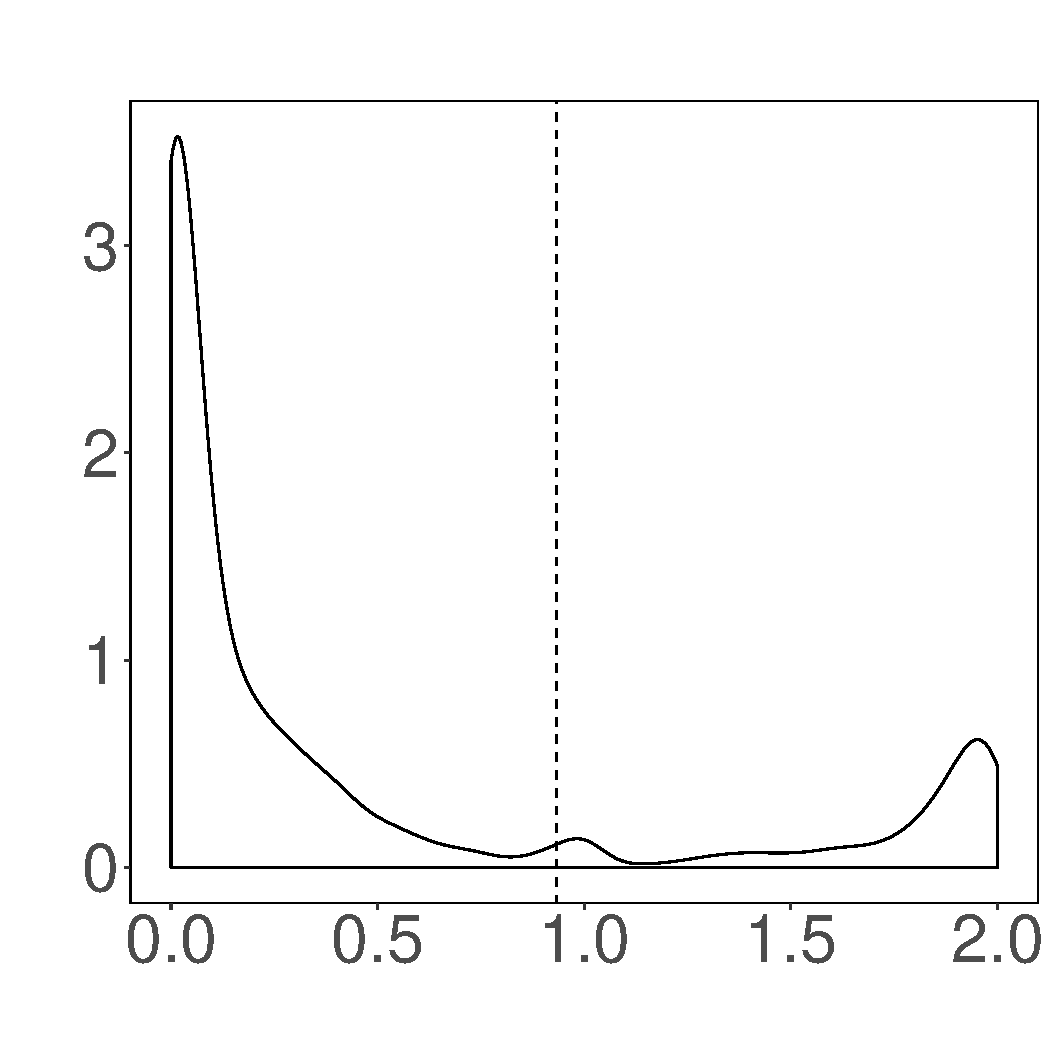
\includegraphics[width=\linewidth]{Figures/cpu-hadoop-cluster.pdf}
                \caption{CPU}
        \end{subfigure}%
        \begin{subfigure}{0.19\textwidth}
                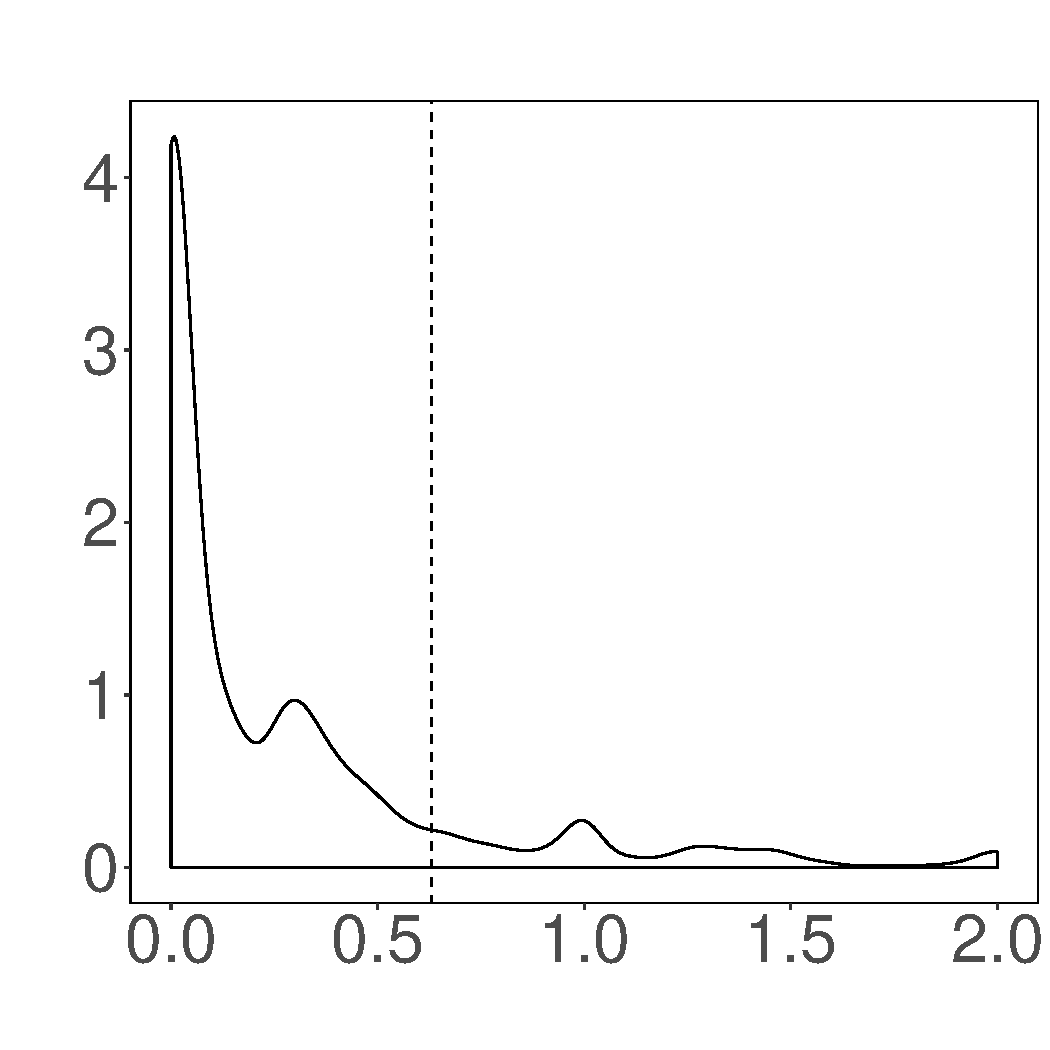
\includegraphics[width=\linewidth]{Figures/mem-hadoop-cluster.pdf}
                \caption{Memory}
        \end{subfigure}%
        \begin{subfigure}{0.19\textwidth}
                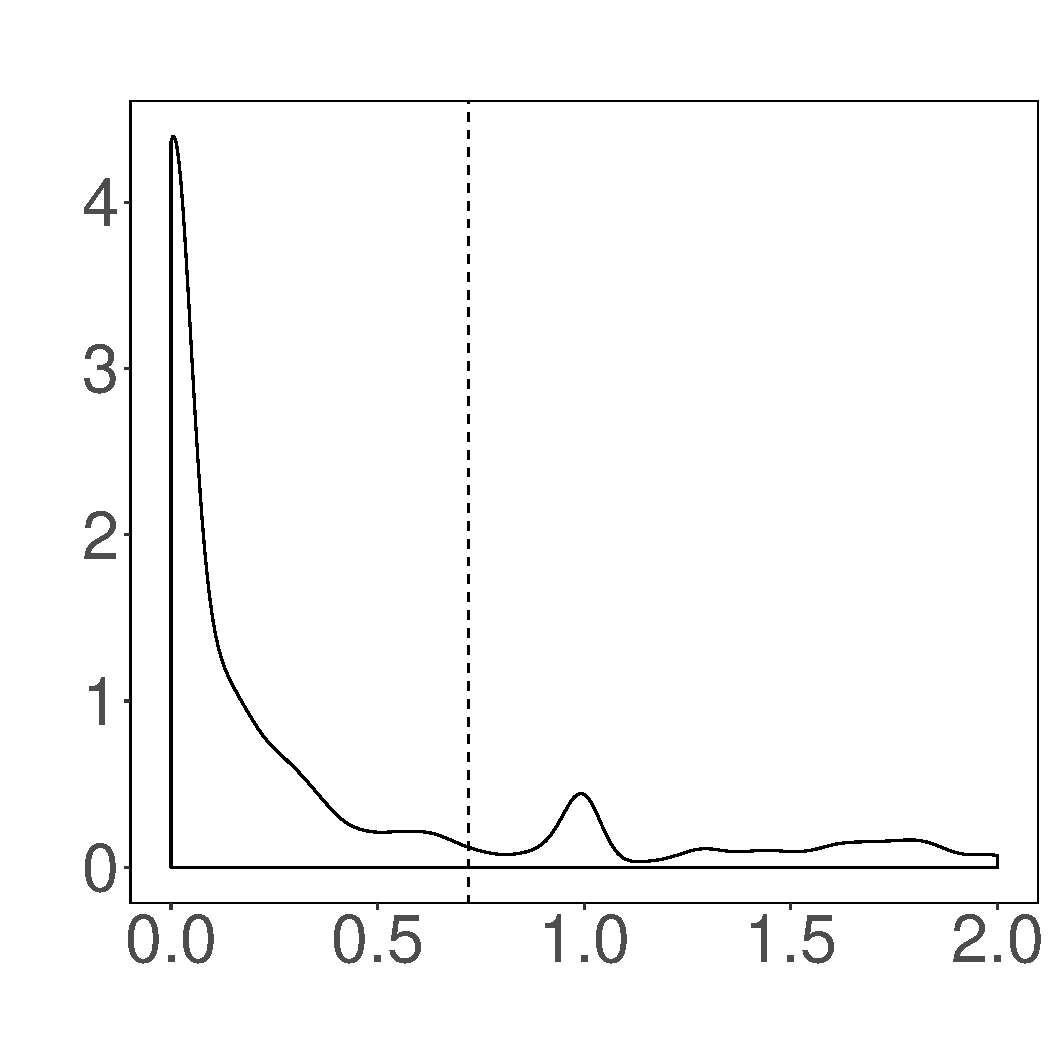
\includegraphics[width=\linewidth]{Figures/ioread-hadoop-cluster.pdf}
                \caption{I/O read}
        \end{subfigure}
        \begin{subfigure}{0.19\textwidth}
                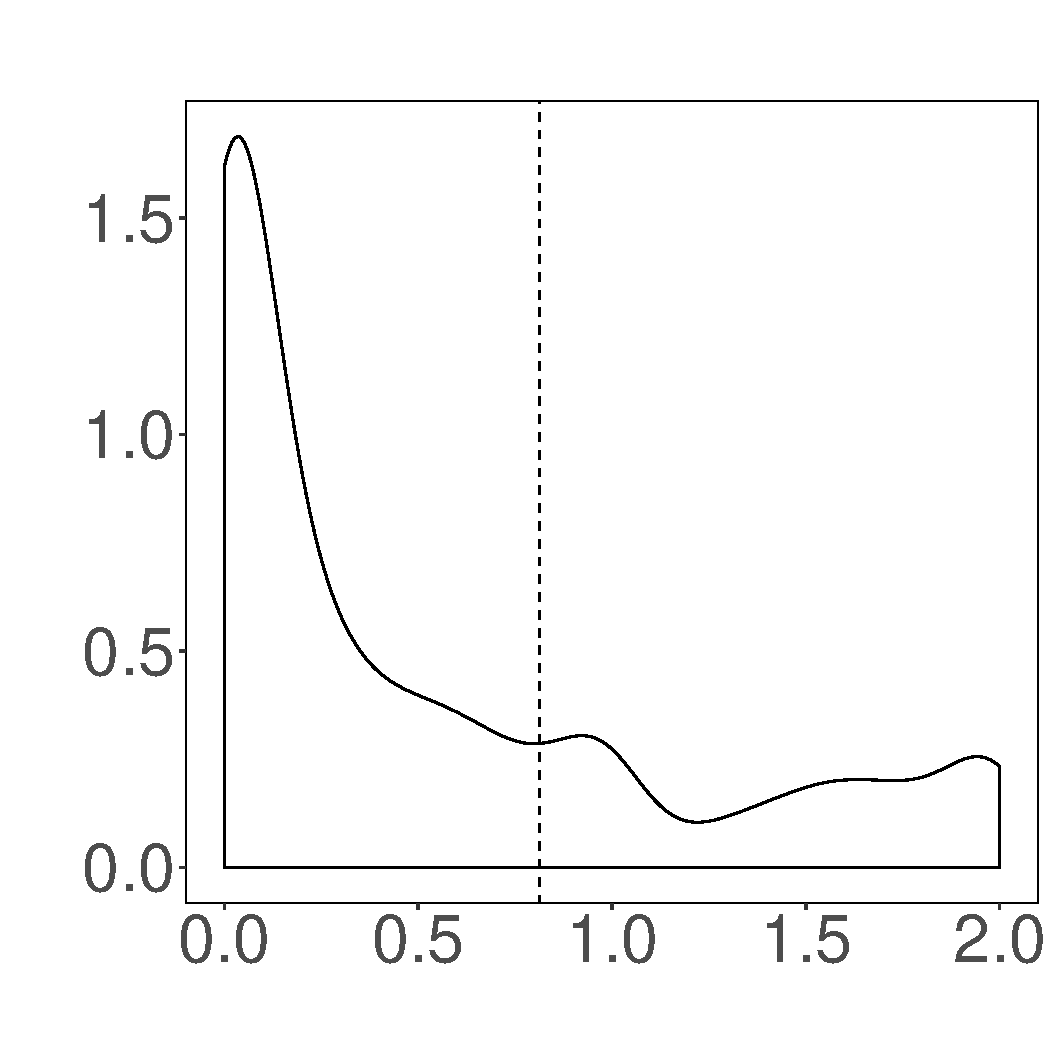
\includegraphics[width=\linewidth]{Figures/iowrite-hadoop-cluster.pdf}
                \caption{I/O write}
        \end{subfigure}
        
	\caption{The automatically obtained thresholds for splitting option variation into \inconsistent and non-\inconsistent groups for \emph{Hadoop}.} % \med{Canssadra or Hadoop? Both fig. 3 and fig. 4 showed Hadoop}.}
	\label{fig:threshold_hadoop}
\end{figure*}

\begin{figure*}%[t]
	\centering
        \begin{subfigure}{0.19\textwidth}
                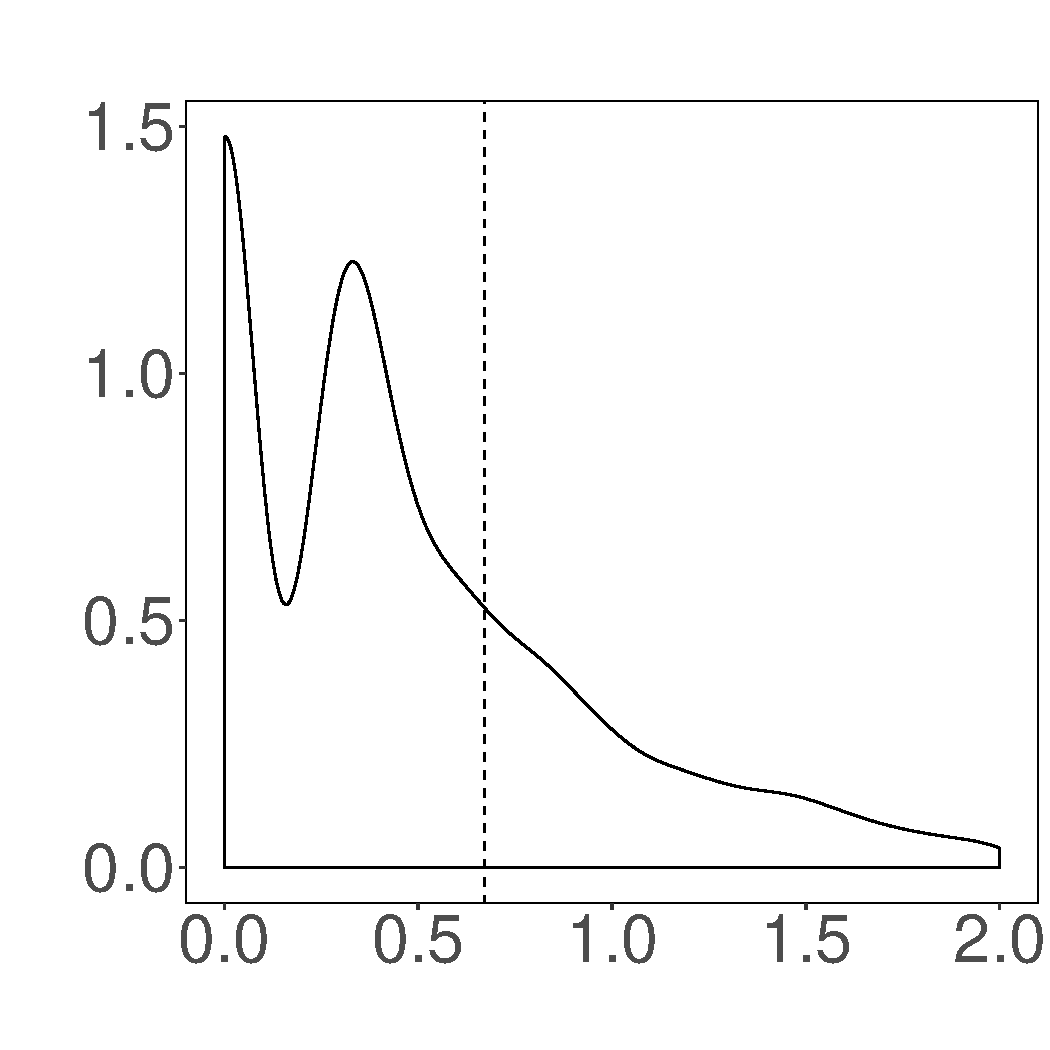
\includegraphics[width=\linewidth]{Figures/runtime-cassandra-cluster.pdf}
                \caption{Res. time}
        \end{subfigure}%
        \begin{subfigure}{0.19\textwidth}
                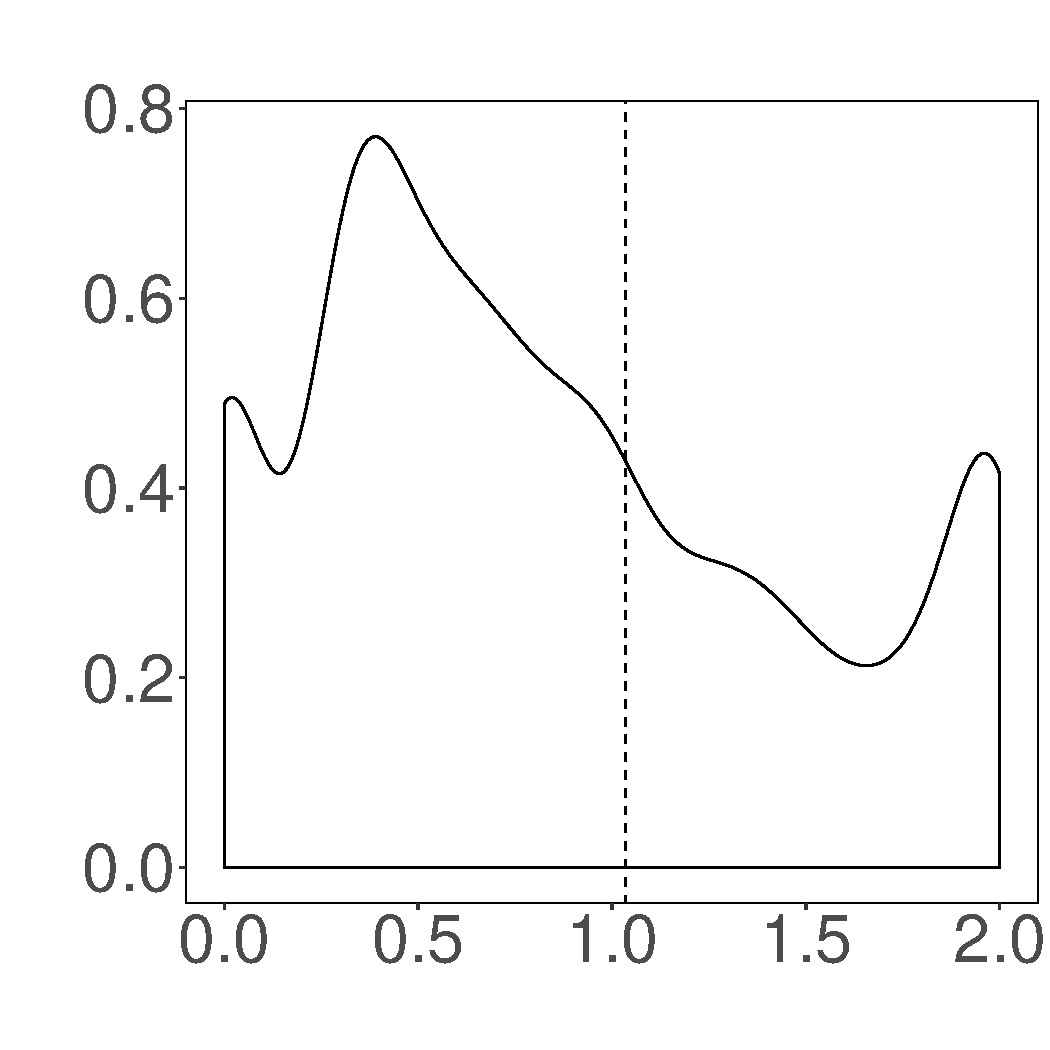
\includegraphics[width=\linewidth]{Figures/cpu-cassandra-cluster.pdf}
                \caption{CPU}
        \end{subfigure}%
        \begin{subfigure}{0.19\textwidth}
                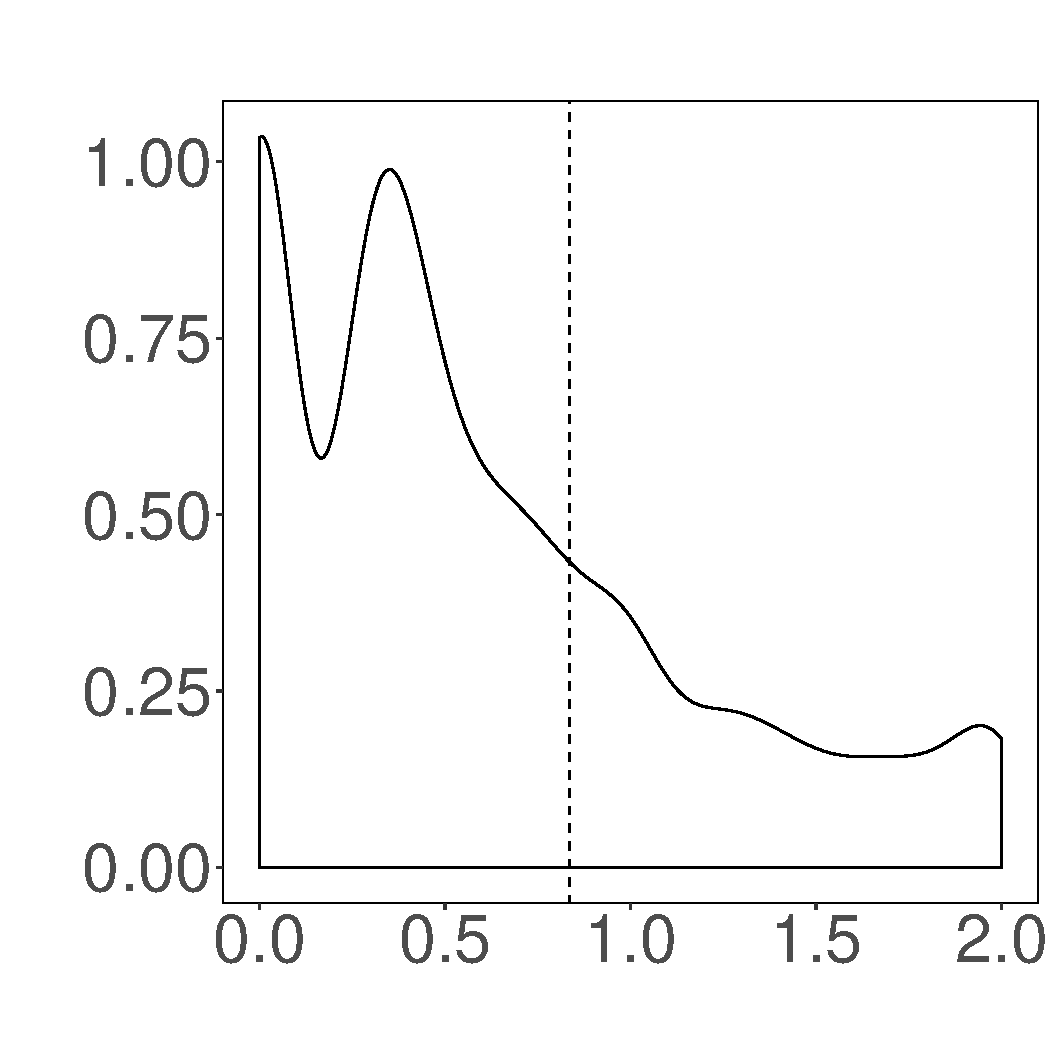
\includegraphics[width=\linewidth]{Figures/mem-cassandra-cluster.pdf}
                \caption{Memory}
        \end{subfigure}%
        \begin{subfigure}{0.19\textwidth}
                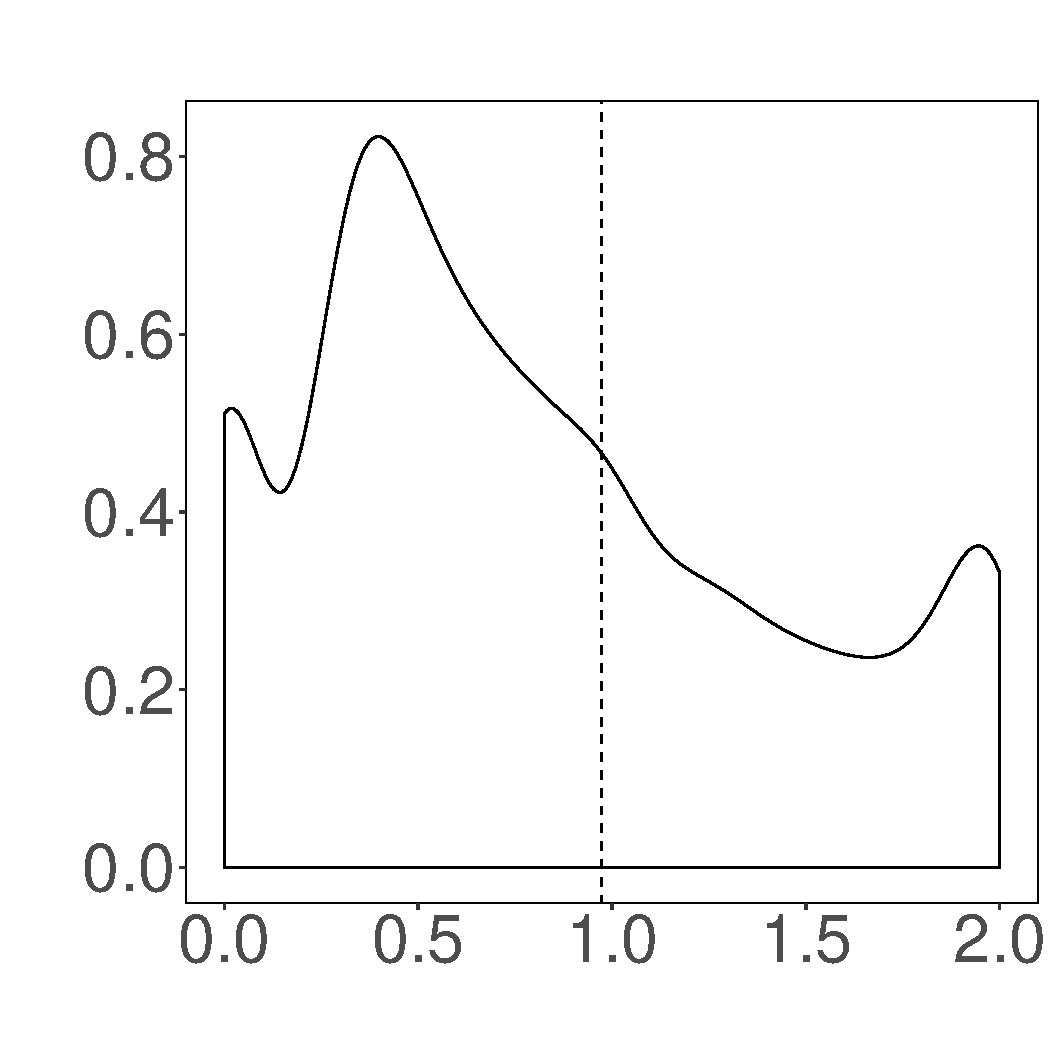
\includegraphics[width=\linewidth]{Figures/ioread-cassandra-cluster.pdf}
                \caption{I/O read}
        \end{subfigure}
        \begin{subfigure}{0.19\textwidth}
                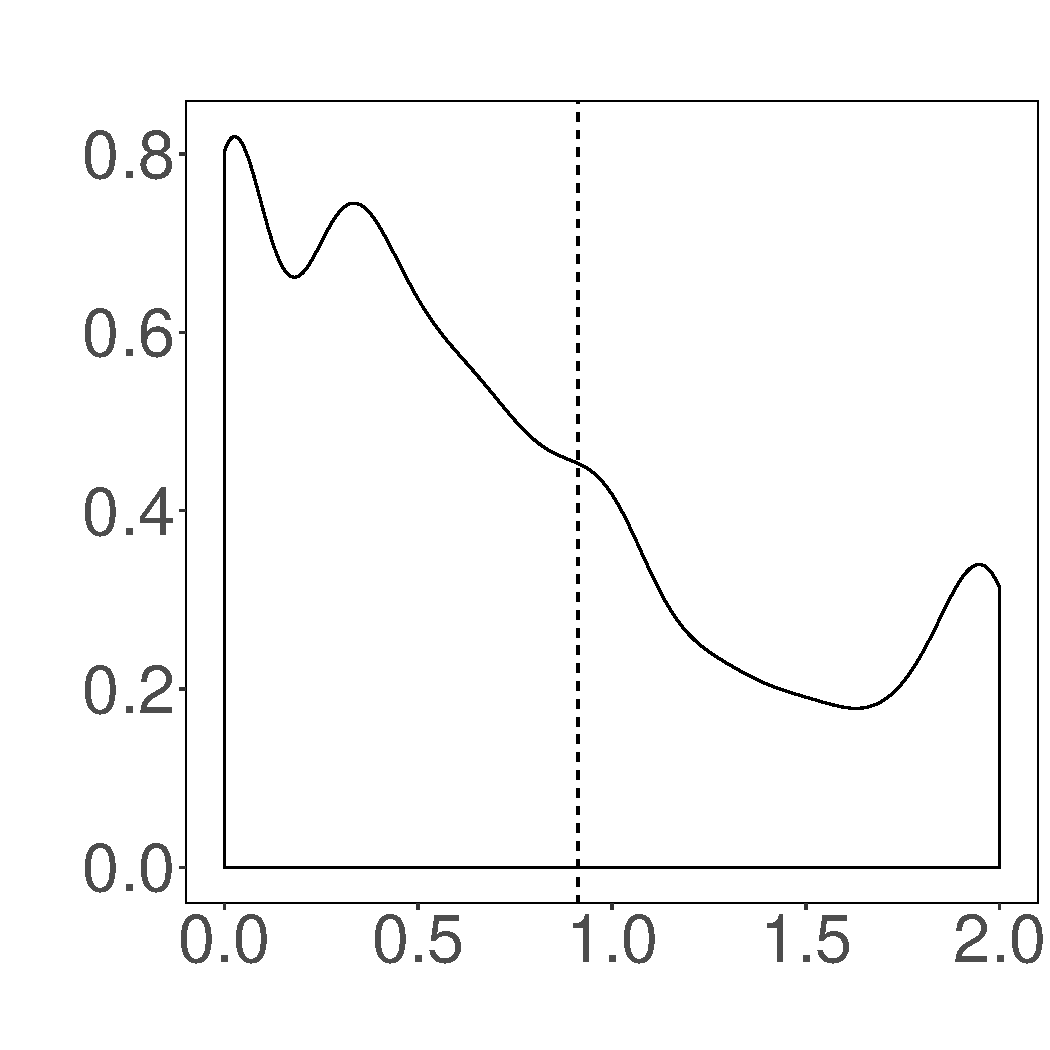
\includegraphics[width=\linewidth]{Figures/iowrite-cassandra-cluster.pdf}
                \caption{I/O write}
        \end{subfigure}
        
	\caption{The automatically obtained thresholds for splitting option variation into \inconsistent and non-\inconsistent groups for \emph{Cassandra}.} % \med{Canssadra or Hadoop? Both fig. 3 and fig. 4 showed Hadoop}.}
	
	\label{fig:threshold\_cassandra}
% 	\vspace{-0.15cm}
\end{figure*}


\begin{figure*}[t]
	\centering
        \begin{subfigure}{0.19\textwidth}
                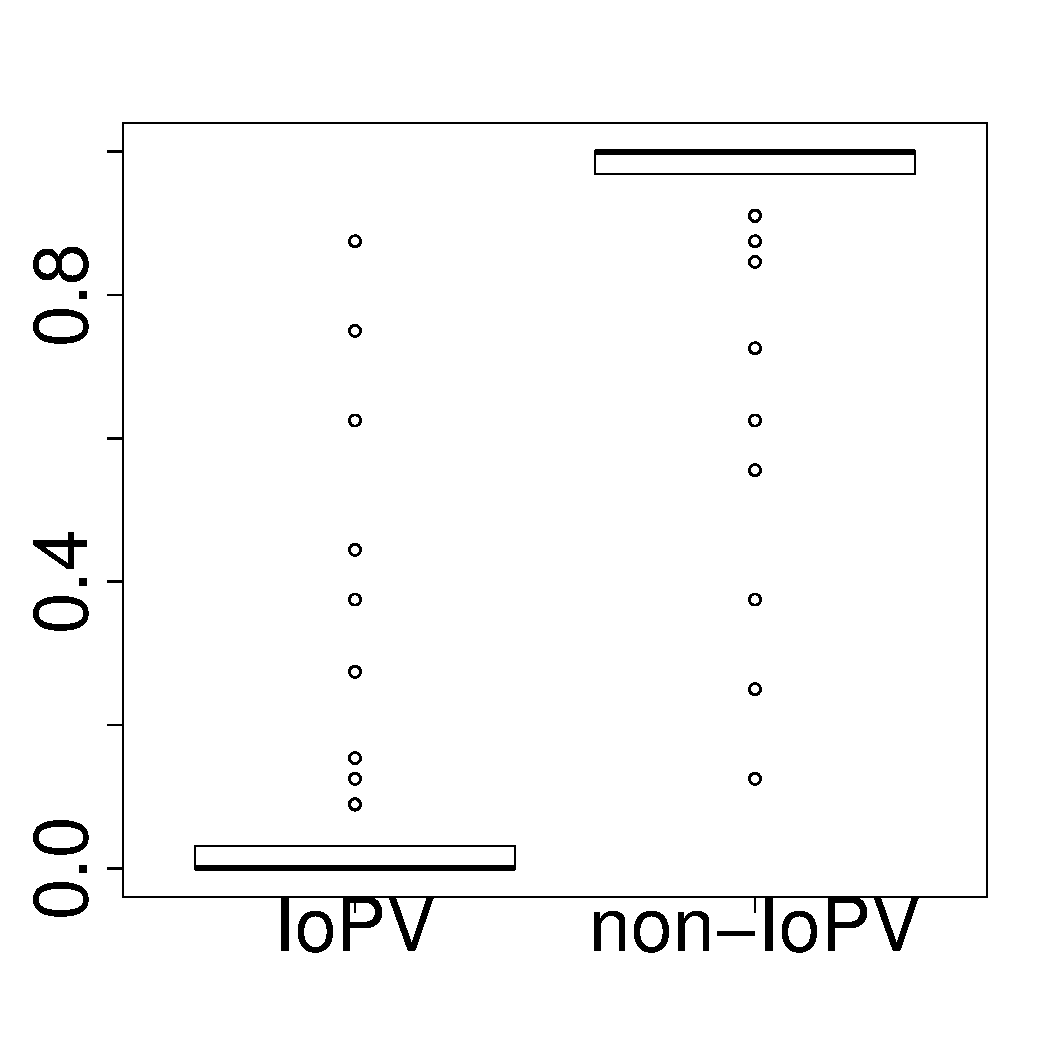
\includegraphics[width=\linewidth]{Figures/runtime-hadoop-boxplot.pdf}
                \caption{Res. time}
        \end{subfigure}%
        \begin{subfigure}{0.19\textwidth}
                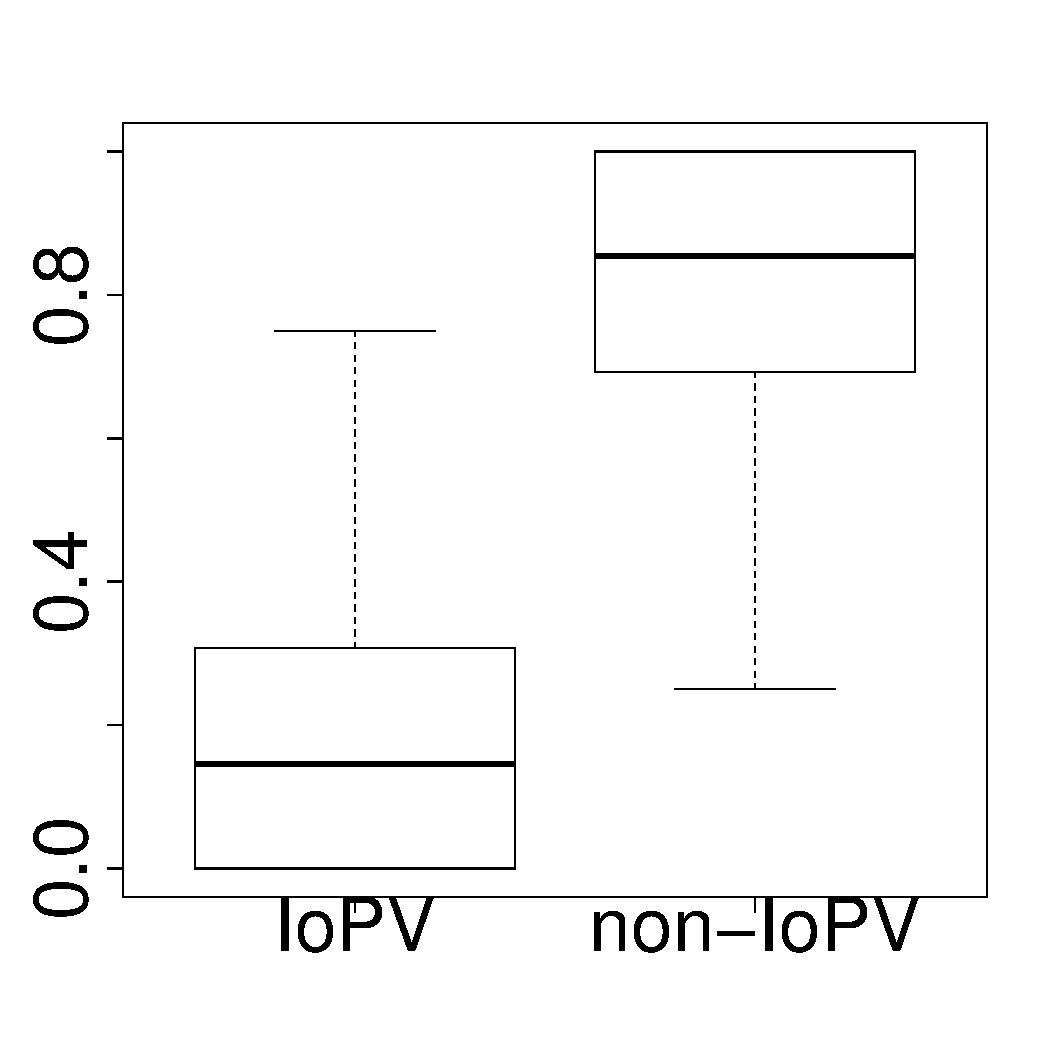
\includegraphics[width=\linewidth]{Figures/cpu-hadoop-boxplot.pdf}
                \caption{CPU}
        \end{subfigure}%
        \begin{subfigure}{0.19\textwidth}
                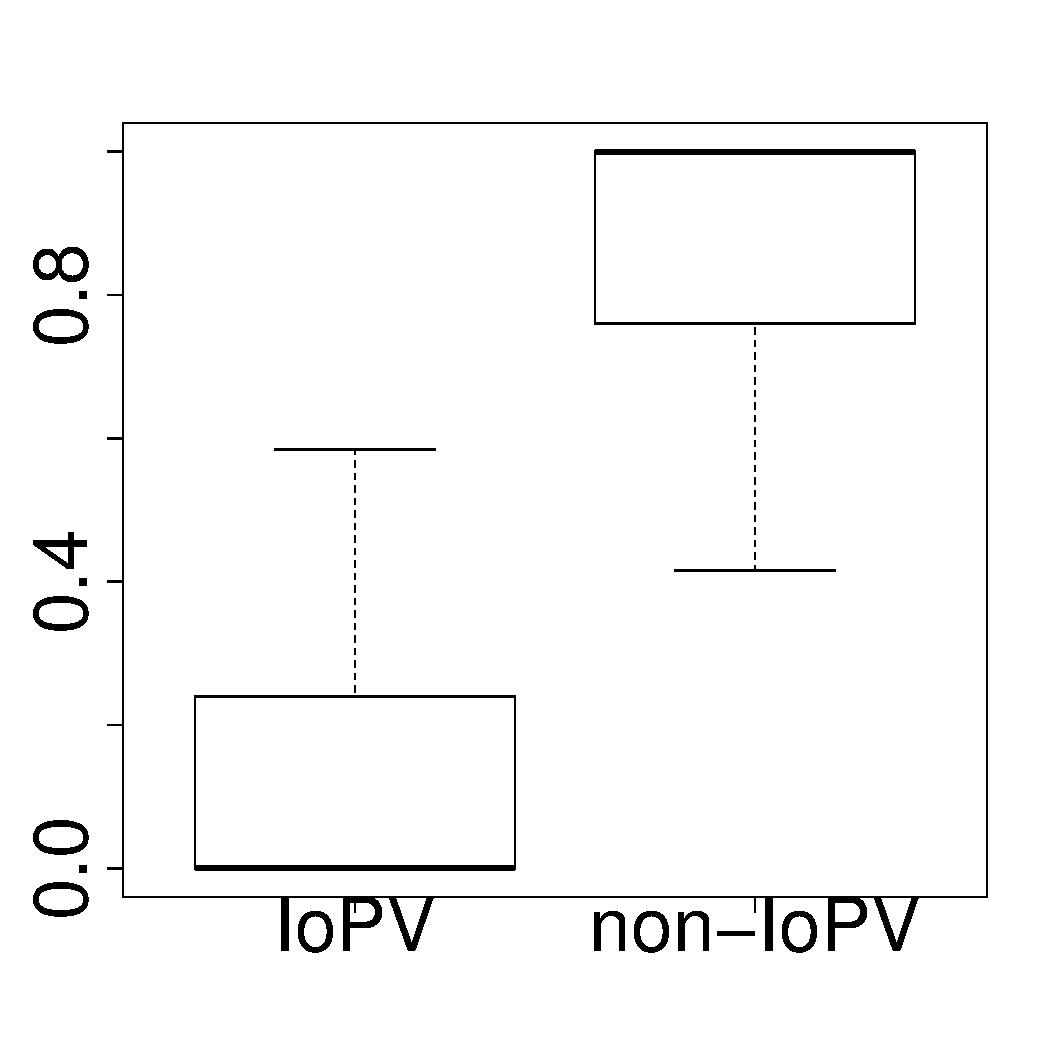
\includegraphics[width=\linewidth]{Figures/mem-hadoop-boxplot.pdf}
                \caption{Memory}
        \end{subfigure}%
        \begin{subfigure}{0.19\textwidth}
                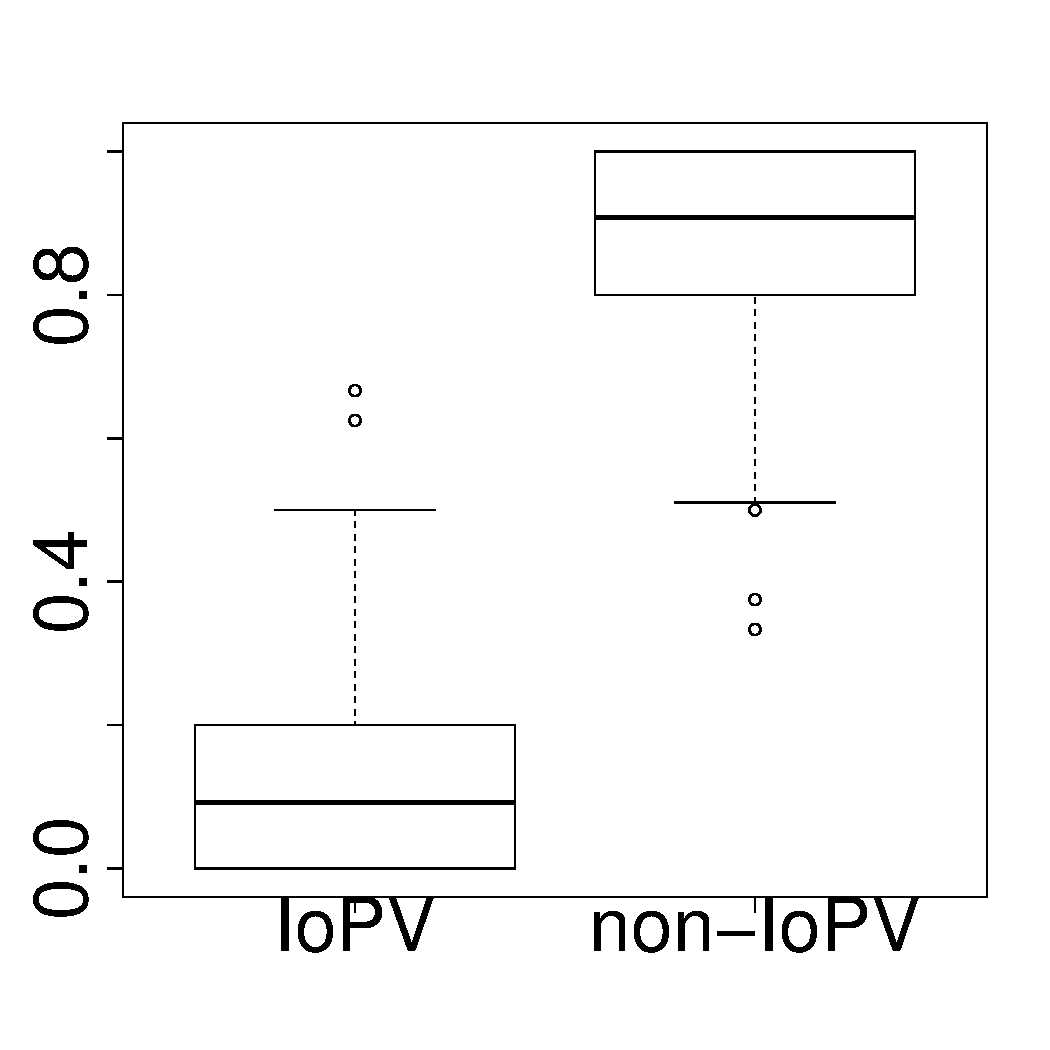
\includegraphics[width=\linewidth]{Figures/ioread-hadoop-boxplot.pdf}
                \caption{I/O read}
        \end{subfigure}
        \begin{subfigure}{0.19\textwidth}
                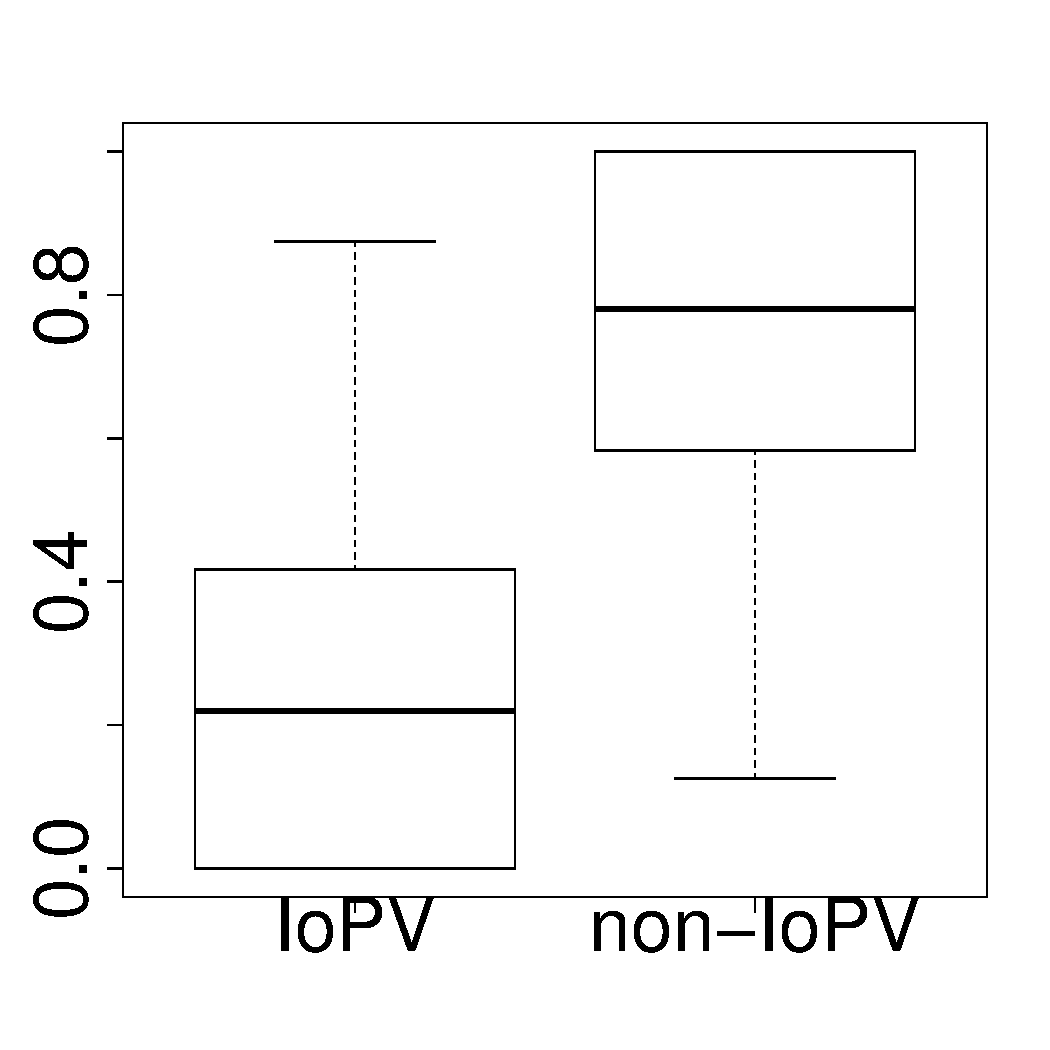
\includegraphics[width=\linewidth]{Figures/iowrite-hadoop-boxplot.pdf}
                \caption{I/O write}
        \end{subfigure}
        
	\caption{Percentage of \inconsistent for each commit of \emph{Hadoop}. Non-\inconsistent is equal to 1-\inconsistent.} %\bram{do we need the non-IoPV boxplots, or are they just 1 minus the IoPV boxplots?}}
	\label{fig:iopv_per_commit_hadoop}
% 	\vspace{-0.15cm}
\end{figure*}

\begin{figure*}[t]
	\centering
        \begin{subfigure}{0.19\textwidth}
                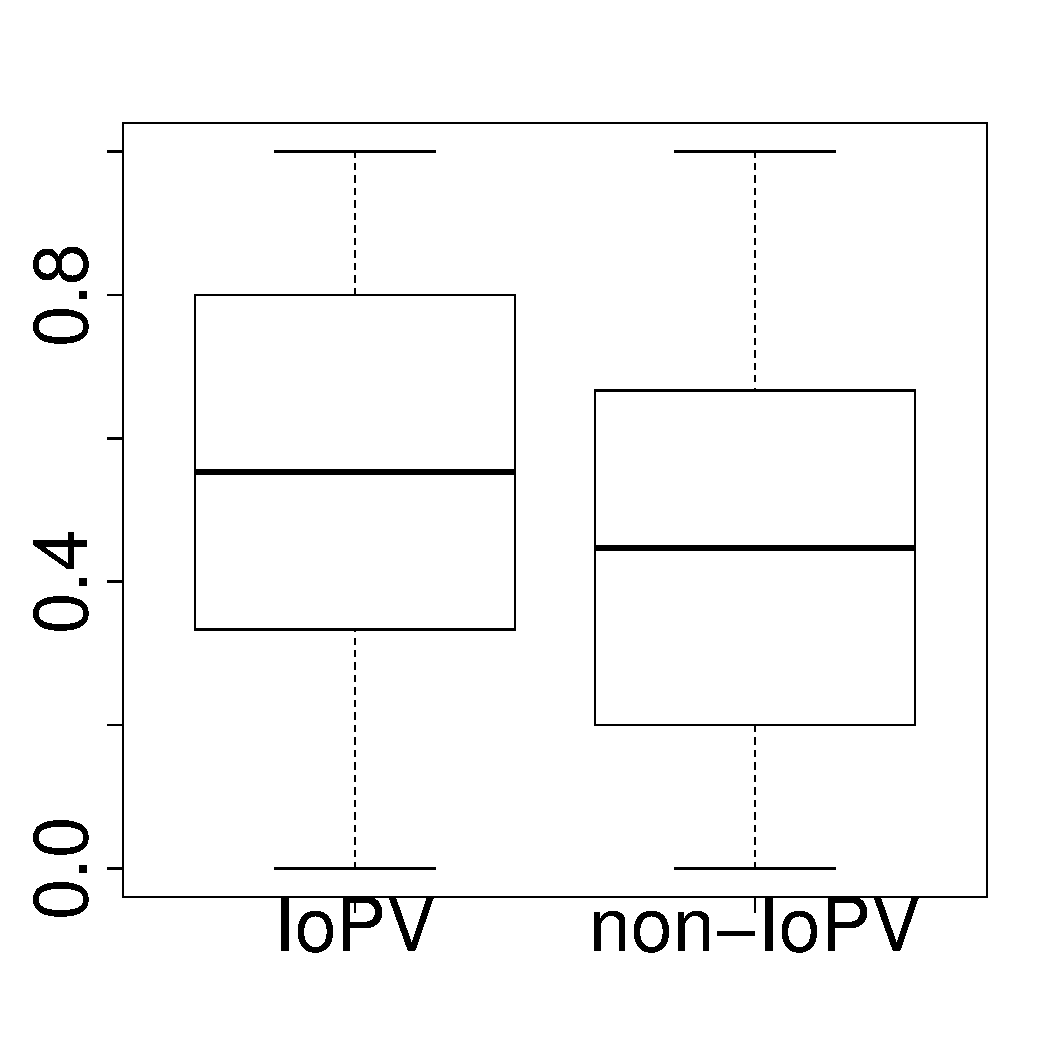
\includegraphics[width=\linewidth]{Figures/runtime-cassandra-boxplot.pdf}
                \caption{Res. time}
        \end{subfigure}%
        \begin{subfigure}{0.19\textwidth}
                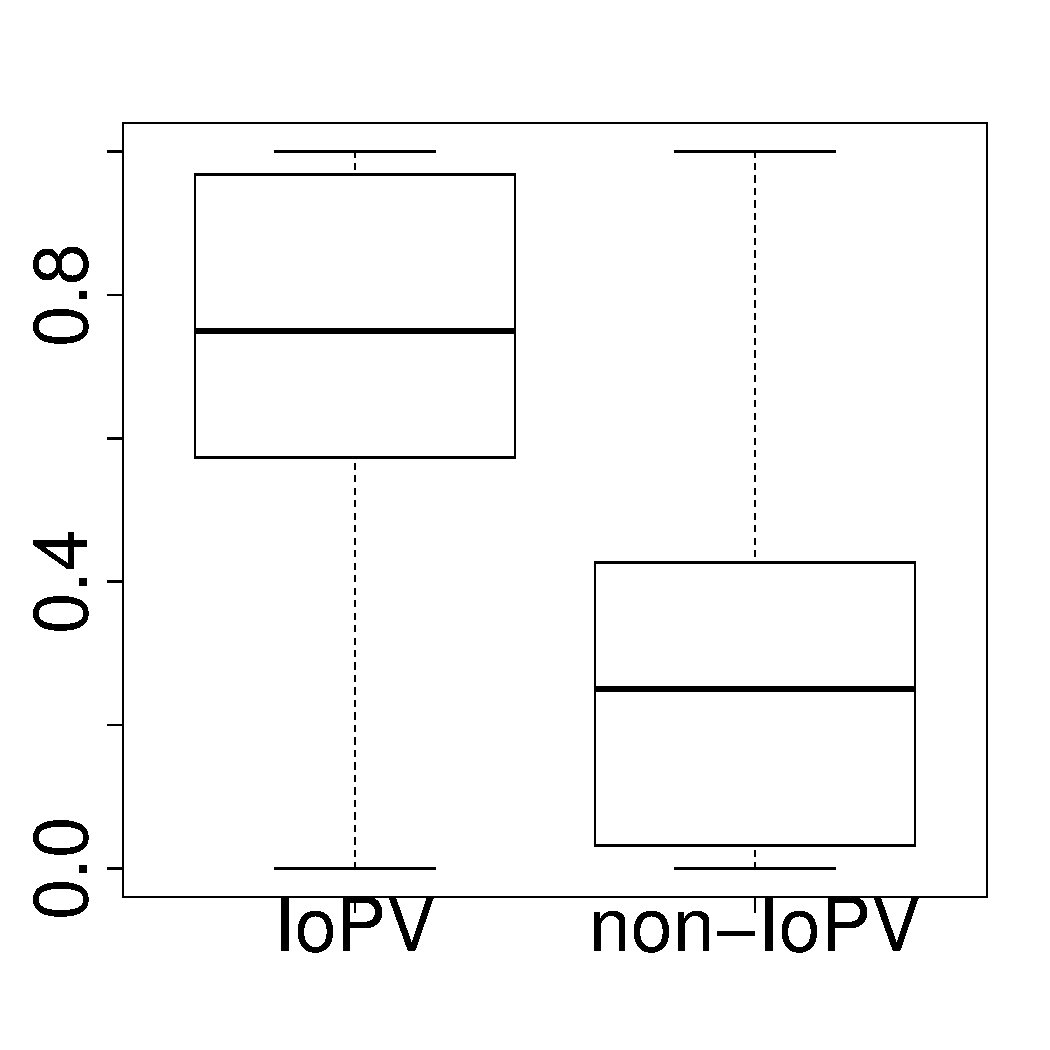
\includegraphics[width=\linewidth]{Figures/cpu-cassandra-boxplot.pdf}
                \caption{CPU}
        \end{subfigure}%
        \begin{subfigure}{0.19\textwidth}
                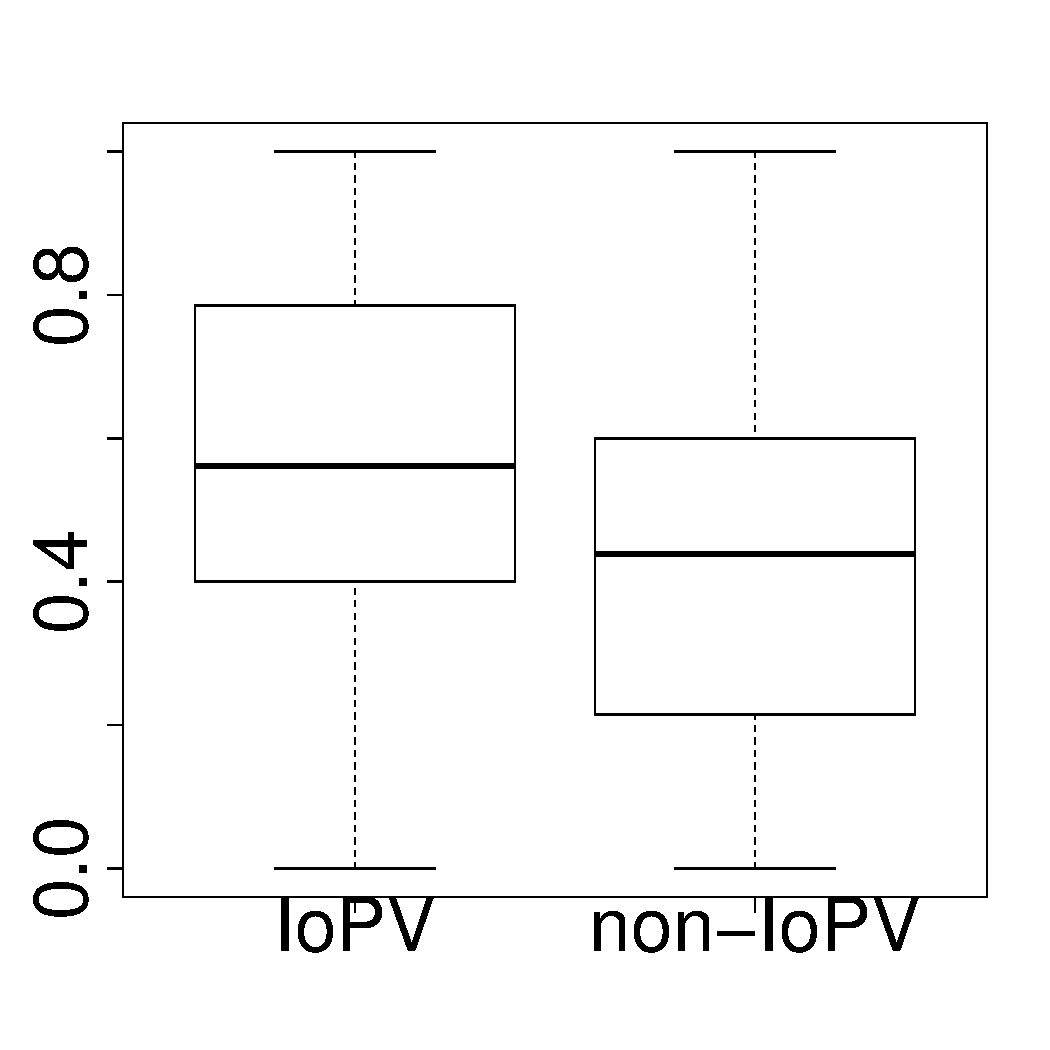
\includegraphics[width=\linewidth]{Figures/mem-cassandra-boxplot.pdf}
                \caption{Memory}
        \end{subfigure}%
        \begin{subfigure}{0.19\textwidth}
                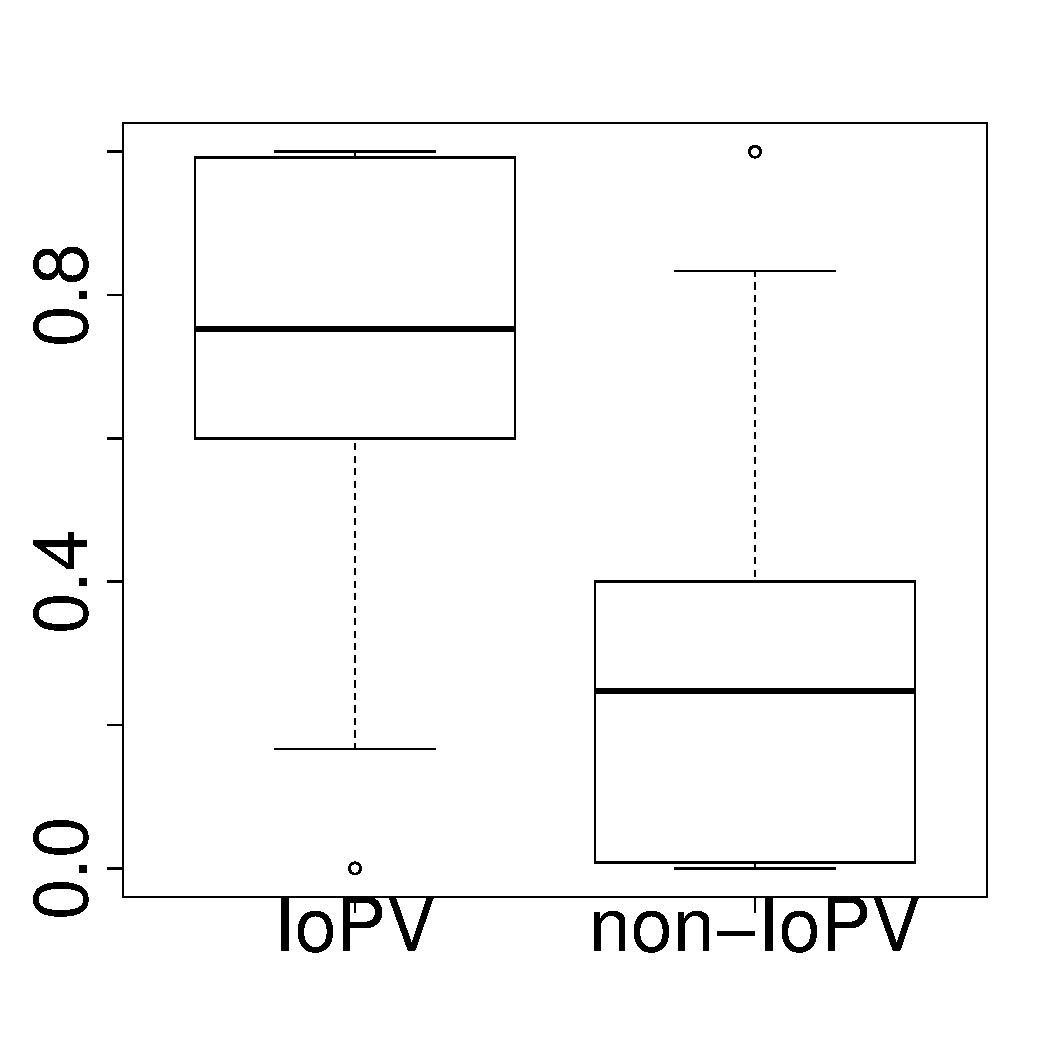
\includegraphics[width=\linewidth]{Figures/ioread-cassandra-boxplot.pdf}
                \caption{I/O read}
        \end{subfigure}
        \begin{subfigure}{0.19\textwidth}
                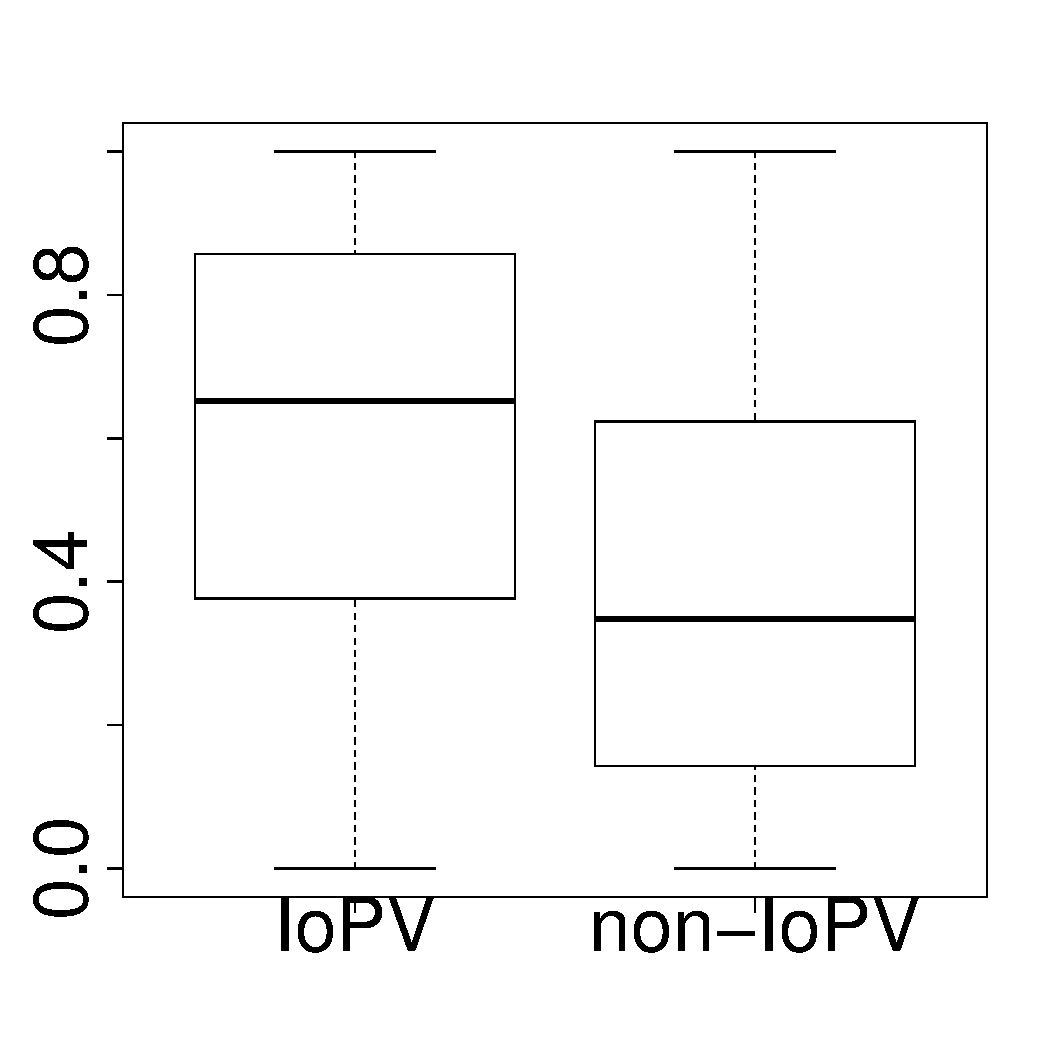
\includegraphics[width=\linewidth]{Figures/iowrite-cassandra-boxplot.pdf}
                \caption{I/O write}
        \end{subfigure}
        
	\caption{Percentage of \inconsistent for each commit of \emph{Cassandra}.  Non-\inconsistent is equal to 1-\inconsistent.} %\bram{do we need the non-IoPV boxplots, or are they just 1 minus the IoPV boxplots?}}
	\label{fig:iopv_per_commit_cassandra}
% 	\vspace{-0.15cm}
\end{figure*}



%\heng{update the numbers}
%\heng{We only keep AUC in the paper and put all metrics in the replication package.}
\begin{table*}
\centering
%\scriptsize
% \tabcolsep=0.08cm
\caption{\emph{Hadoop}'s results of using different models to predict whether configuration options cause the manifesting of \inconsistent. The best results for each performance metric and each model are highlighted in \textit{italic}. The best results for each performance metric across different models are highlighted in \textbf{\textit{bold-italic}}.} %\heng{Still a few results show very low precision and recall but high AUC (e.g., NN with tf-idf on Hadoop for Res. time and CPU, CNN with tf-idf on Hadoop for CPU} \heng{Todo: only keep AUC} \jinfu{Update Table6 and Table7}}

\begin{tabular}{|c|r|r|r|r|r|r|r|r|r|}
\hline
\multicolumn{10}{|c|}{Hadoop}    \\ \hline
\multirow{2}{*}{} & \multicolumn{3}{c|}{RF with tf-idf}        & \multicolumn{3}{c|}{RF with PCA}           & \multicolumn{3}{c|}{RF with code embedding}\\ \cline{2-10} 
                  & \multicolumn{1}{c|}{Pre.} & \multicolumn{1}{c|}{Recall} & \multicolumn{1}{c|}{AUC} & \multicolumn{1}{c|}{Pre.} & \multicolumn{1}{c|}{Recall} & \multicolumn{1}{c|}{AUC} & \multicolumn{1}{c|}{Pre.} & \multicolumn{1}{c|}{Recall} & \multicolumn{1}{c|}{AUC} \\ \hline
Res. time         & 0.68  & 0.39    & \textit{0.93}            & 0.68  & 0.39    & 0.66 & 0.73  & 0.33    & \textit{0.93}            \\ \hline
Cpu               & 0.70  & 0.51    & 0.90 & 0.55  & 0.02    & 0.71 & 0.77  & 0.60    & \textit{\textbf{0.92}}   \\ \hline
Memory            & 0.64  & 0.36    & 0.87 & 0.48  & 0.04    & 0.69 & 0.75  & 0.41    & \textit{\textbf{0.91}}   \\ \hline
I/O Read          & 0.68  & 0.54    & 0.91 & 0.58  & 0.02    & 0.76 & 0.79  & 0.56    & \textit{\textbf{0.93}}   \\ \hline
I/O Write         & 0.63  & 0.44    & 0.82 & 0.44  & 0.02    & 0.59 & 0.72  & 0.49    & \textit{\textbf{0.85}}   \\ \hline
Average           & 0.67  & 0.45    & 0.89 & 0.55  & 0.10    & 0.68 & 0.75  & 0.48    & \textit{\textbf{0.91}}   \\ \hline
\multirow{2}{*}{} & \multicolumn{3}{c|}{LR with tf-idf}        & \multicolumn{3}{c|}{LR with PCA}           & \multicolumn{3}{c|}{LR with code embedding}\\ \cline{2-10} 
                  & \multicolumn{1}{c|}{Pre.} & \multicolumn{1}{c|}{Recall} & \multicolumn{1}{c|}{AUC} & \multicolumn{1}{c|}{Pre.} & \multicolumn{1}{c|}{Recall} & \multicolumn{1}{c|}{AUC} & \multicolumn{1}{c|}{Pre.} & \multicolumn{1}{c|}{Recall} & \multicolumn{1}{c|}{AUC} \\ \hline
Res. time         & 0.38  & 0.03    & 0.67 & 0.12  & 0.46    & 0.54 & 0.53  & 0.09    & \textit{0.77}            \\ \hline
Cpu               & 0.66  & 0.06    & 0.73 & 0.27  & 0.29    & 0.61 & 0.48  & 0.14    & \textit{0.76}            \\ \hline
Memory            & 0.49  & 0.04    & 0.71 & 0.16  & 0.40    & 0.55 & 0.48  & 0.10    & \textit{0.73}            \\ \hline
I/O Read          & 0.70  & 0.05    & 0.71 & 0.22  & 0.33    & 0.57 & 0.46  & 0.18    & \textit{0.80}            \\ \hline
I/O Write         & 0.50  & 0.06    & 0.64 & 0.33  & 0.22    & 0.57 & 0.50  & 0.14    & \textit{0.66}            \\ \hline
Average           & 0.55  & 0.05    & 0.69 & 0.22  & 0.34    & 0.57 & 0.49  & 0.13    & \textit{0.74}            \\ \hline
\multirow{2}{*}{} & \multicolumn{3}{c|}{XG with tf-idf}        & \multicolumn{3}{c|}{XG with PCA}           & \multicolumn{3}{c|}{XG with code embedding}\\ \cline{2-10} 
                  & \multicolumn{1}{c|}{Pre.} & \multicolumn{1}{c|}{Recall} & \multicolumn{1}{c|}{AUC} & \multicolumn{1}{c|}{Pre.} & \multicolumn{1}{c|}{Recall} & \multicolumn{1}{c|}{AUC} & \multicolumn{1}{c|}{Pre.} & \multicolumn{1}{c|}{Recall} & \multicolumn{1}{c|}{AUC} \\ \hline
Res. time         & 0.65  & 0.42    & \textit{\textbf{0.94}}   & 1.00  & 0.05    & 0.60 & 0.71  & 0.31    & 0.93 \\ \hline
Cpu               & 0.66  & 0.48    & \textit{0.88}            & 0.32  & 0.06    & 0.62 & 0.67  & 0.50    & \textit{0.88}            \\ \hline
Memory            & 0.66  & 0.32    & \textit{0.87}            & 0.41  & 0.04    & 0.68 & 0.72  & 0.32    & \textit{0.87}            \\ \hline
I/O Read          & 0.66  & 0.49    & \textit{0.91}            & 0.49  & 0.08    & 0.73 & 0.73  & 0.50    & \textit{0.91}            \\ \hline
I/O Write         & 0.66  & 0.38    & \textit{0.82}            & 0.41  & 0.16    & 0.58 & 0.67  & 0.40    & 0.80 \\ \hline
Average           & 0.66  & 0.42    & \textit{0.88}            & 0.52  & 0.08    & 0.64 & 0.70  & 0.41    & 0.88 \\ \hline
\multirow{2}{*}{} & \multicolumn{3}{c|}{NN with tf-idf}        & \multicolumn{3}{c|}{NN with PCA}           & \multicolumn{3}{c|}{NN with code embedding}\\ \cline{2-10} 
                  & \multicolumn{1}{c|}{Pre.} & \multicolumn{1}{c|}{Recall} & \multicolumn{1}{c|}{AUC} & \multicolumn{1}{c|}{Pre.} & \multicolumn{1}{c|}{Recall} & \multicolumn{1}{c|}{AUC} & \multicolumn{1}{c|}{Pre.} & \multicolumn{1}{c|}{Recall} & \multicolumn{1}{c|}{AUC} \\ \hline
Res. time         & 0.34  & 0.54    & 0.79 & 0.27  & 0.83    & \textit{0.80}            & 0.27  & 0.64    & 0.75 \\ \hline
Cpu               & 0.53  & 0.30    & 0.72 & 0.63  & 0.41    & \textit{0.73}            & 0.39  & 0.33    & 0.65 \\ \hline
Memory            & 0.43  & 0.27    & \textit{0.67}            & 0.52  & 0.34    & \textit{0.67}            & 0.31  & 0.42    & 0.66 \\ \hline
I/O Read          & 0.53  & 0.44    & 0.73 & 0.60  & 0.46    & \textit{0.76}            & 0.48  & 0.33    & 0.72 \\ \hline
I/O Write         & 0.50  & 0.38    & \textit{0.68}            & 0.53  & 0.32    & 0.65 & 0.39  & 0.41    & \textit{0.68}            \\ \hline
Average           & 0.47  & 0.39    & \textit{0.72}            & 0.51  & 0.47    & \textit{0.72}            & 0.37  & 0.43    & 0.69 \\ \hline
\multirow{2}{*}{} & \multicolumn{3}{c|}{CNN with tf-idf}       & \multicolumn{3}{c|}{CNN with PCA}          & \multicolumn{3}{c|}{CNN with code embedding}                   \\ \cline{2-10} 
                  & \multicolumn{1}{c|}{Pre.} & \multicolumn{1}{c|}{Recall} & \multicolumn{1}{c|}{AUC} & \multicolumn{1}{c|}{Pre.} & \multicolumn{1}{c|}{Recall} & \multicolumn{1}{c|}{AUC} & \multicolumn{1}{c|}{Pre.} & \multicolumn{1}{c|}{Recall} & \multicolumn{1}{c|}{AUC} \\ \hline
Res. time         & 0.29  & 0.48    & 0.75 & 0.06  & 0.90    & 0.73 & 0.23  & 0.51    & \textit{0.79}            \\ \hline
Cpu               & 0.22  & 0.68    & 0.78 & 0.18  & 0.78    & 0.76 & 0.63  & 0.25    & \textit{0.81}            \\ \hline
Memory            & 0.47  & 0.25    & 0.69 & 0.13  & 0.87    & 0.74 & 0.20  & 0.57    & \textit{0.76}            \\ \hline
I/O Read          & 0.32  & 0.41    & \textit{0.68}            & 0.27  & 0.25    & \textit{0.68}            & 0.20  & 0.38    & 0.66 \\ \hline
I/O Write         & 0.27  & 0.31    & 0.64 & 0.14  & 0.64    & 0.65 & 0.19  & 0.60    & \textit{0.67}            \\ \hline
Average           & 0.31  & 0.43    & 0.71 & 0.16  & 0.69    & 0.71 & 0.29  & 0.46    & \textit{0.74}            \\ \hline
\end{tabular}

\label{tab:model_evaluation_hadoop}
\end{table*}




\begin{table*}
\centering
%\tabcolsep=0.08cm
%\scriptsize
\caption{\emph{Cassandra}'s results of using different models to predict whether configuration options cause the manifesting of \inconsistent. The best results for each performance metric and each model are highlighted in \textit{italic}. The best results for each performance metric across different models are highlighted in \textbf{\textit{bold-italic}}.}
\begin{tabular}{|c|r|r|r|r|r|r|r|r|r|}
\hline
\multicolumn{10}{|c|}{Cassandra}          \\ \hline
\multirow{2}{*}{} & \multicolumn{3}{c|}{RF with tf-idf}      & \multicolumn{3}{c|}{RF with PCA}         & \multicolumn{3}{c|}{RF with code embedding}                   \\ \cline{2-10} 
                  & \multicolumn{1}{c|}{Pre.} & \multicolumn{1}{c|}{Recall} & \multicolumn{1}{c|}{AUC} & \multicolumn{1}{c|}{Pre.} & \multicolumn{1}{c|}{Recall} & \multicolumn{1}{c|}{AUC} & \multicolumn{1}{c|}{Pre.} & \multicolumn{1}{c|}{Recall} & \multicolumn{1}{c|}{AUC} \\ \hline
Res. time         & 0.74 & 0.37   & 0.74& 0.45 & 0.13   & 0.62& 0.67 & 0.46   & \textit{0.75}            \\ \hline
Cpu               & 0.68 & 0.39   & 0.76& 0.46 & 0.15   & 0.61& 0.73 & 0.59   & \textit{0.82}            \\ \hline
Memory            & 0.71 & 0.37   & 0.78& 0.35 & 0.04   & 0.61& 0.71 & 0.58   & \textit{\textbf{0.84}}   \\ \hline
I/O Read          & 0.74 & 0.48   & 0.79& 0.54 & 0.32   & 0.67& 0.74 & 0.63   & \textit{\textbf{0.83}}   \\ \hline
I/O Write         & 0.76 & 0.50   & 0.82& 0.58 & 0.32   & 0.68& 0.77 & 0.65   & \textit{\textbf{0.86}}   \\ \hline
Average           & 0.73 & 0.42   & 0.78& 0.47 & 0.19   & 0.64& 0.72 & 0.58   & \textit{0.82}            \\ \hline
\multirow{2}{*}{} & \multicolumn{3}{c|}{LR with tf-idf}      & \multicolumn{3}{c|}{LR with PCA}         & \multicolumn{3}{c|}{LR with code embedding}                   \\ \cline{2-10} 
                  & \multicolumn{1}{c|}{Pre.} & \multicolumn{1}{c|}{Recall} & \multicolumn{1}{c|}{AUC} & \multicolumn{1}{c|}{Pre.} & \multicolumn{1}{c|}{Recall} & \multicolumn{1}{c|}{AUC} & \multicolumn{1}{c|}{Pre.} & \multicolumn{1}{c|}{Recall} & \multicolumn{1}{c|}{AUC} \\ \hline
Res. time         & 0.38 & 0.38   & 0.59& 0.28 & 0.54   & 0.54& 0.38 & 0.51   & \textit{0.63}            \\ \hline
Cpu               & 0.49 & 0.42   & 0.64& 0.33 & 0.41   & 0.53& 0.46 & 0.58   & \textit{0.65}            \\ \hline
Memory            & 0.44 & 0.26   & 0.62& 0.29 & 0.28   & 0.55& 0.43 & 0.47   & \textit{0.66}            \\ \hline
I/O Read          & 0.50 & 0.50   & 0.63& 0.35 & 0.44   & 0.55& 0.49 & 0.61   & \textit{0.67}            \\ \hline
I/O Write         & 0.53 & 0.51   & \textit{0.69}            & 0.36 & 0.37   & 0.54& 0.47 & 0.63   & 0.68\\ \hline
Average           & 0.47 & 0.41   & 0.64& 0.32 & 0.41   & 0.54& 0.44 & 0.56   & \textit{0.66}            \\ \hline
\multirow{2}{*}{} & \multicolumn{3}{c|}{XG with tf-idf}      & \multicolumn{3}{c|}{XG with PCA}         & \multicolumn{3}{c|}{XG with code embedding}                   \\ \cline{2-10} 
                  & \multicolumn{1}{c|}{Pre.} & \multicolumn{1}{c|}{Recall} & \multicolumn{1}{c|}{AUC} & \multicolumn{1}{c|}{Pre.} & \multicolumn{1}{c|}{Recall} & \multicolumn{1}{c|}{AUC} & \multicolumn{1}{c|}{Pre.} & \multicolumn{1}{c|}{Recall} & \multicolumn{1}{c|}{AUC} \\ \hline
Res. time         & 0.66 & 0.38   & \textit{0.75}            & 0.37 & 0.20   & 0.60& 0.63 & 0.44   & 0.74\\ \hline
Cpu               & 0.65 & 0.49   & 0.77& 0.49 & 0.32   & 0.63& 0.70 & 0.60   & \textit{0.82}            \\ \hline
Memory            & 0.65 & 0.49   & 0.80& 0.45 & 0.13   & 0.60& 0.70 & 0.56   & \textit{0.83}            \\ \hline
I/O Read          & 0.69 & 0.55   & 0.79& 0.46 & 0.35   & 0.61& 0.72 & 0.62   & \textit{0.81}            \\ \hline
I/O Write         & 0.74 & 0.59   & 0.84& 0.48 & 0.33   & 0.65& 0.74 & 0.64   & \textit{0.85}            \\ \hline
Average           & 0.68 & 0.50   & 0.79& 0.45 & 0.27   & 0.62& 0.70 & 0.57   & \textit{0.81}            \\ \hline
\multirow{2}{*}{} & \multicolumn{3}{c|}{NN with tf-idf}      & \multicolumn{3}{c|}{NN with PCA}         & \multicolumn{3}{c|}{NN with code embedding}                   \\ \cline{2-10} 
                  & \multicolumn{1}{c|}{Pre.} & \multicolumn{1}{c|}{Recall} & \multicolumn{1}{c|}{AUC} & \multicolumn{1}{c|}{Pre.} & \multicolumn{1}{c|}{Recall} & \multicolumn{1}{c|}{AUC} & \multicolumn{1}{c|}{Pre.} & \multicolumn{1}{c|}{Recall} & \multicolumn{1}{c|}{AUC} \\ \hline
Res. time         & 0.55 & 0.36   & 0.71& 0.53 & 0.40   & \textit{0.73}            & 0.47 & 0.41   & 0.67\\ \hline
Cpu               & 0.27 & 0.94   & 0.88& 0.31 & 0.96   & \textit{\textbf{0.90}}   & 0.26 & 0.88   & 0.84\\ \hline
Memory            & 0.56 & 0.51   & 0.76& 0.64 & 0.57   & \textit{\textbf{0.84}}   & 0.61 & 0.49   & 0.76\\ \hline
I/O Read          & 0.66 & 0.46   & 0.75& 0.67 & 0.57   & \textit{\textbf{0.83}}   & 0.60 & 0.54   & 0.74\\ \hline
I/O Write         & 0.67 & 0.39   & 0.77& 0.70 & 0.57   & \textit{0.84}            & 0.63 & 0.55   & 0.77\\ \hline
Average           & 0.54 & 0.53   & 0.77& 0.57 & 0.62   & \textit{\textbf{0.83}}   & 0.51 & 0.57   & 0.76\\ \hline
\multirow{2}{*}{} & \multicolumn{3}{c|}{CNN with tf-idf}     & \multicolumn{3}{c|}{CNN with PCA}        & \multicolumn{3}{c|}{CNN with code embedding}                  \\ \cline{2-10} 
                  & \multicolumn{1}{c|}{Pre.} & \multicolumn{1}{c|}{Recall} & \multicolumn{1}{c|}{AUC} & \multicolumn{1}{c|}{Pre.} & \multicolumn{1}{c|}{Recall} & \multicolumn{1}{c|}{AUC} & \multicolumn{1}{c|}{Pre.} & \multicolumn{1}{c|}{Recall} & \multicolumn{1}{c|}{AUC} \\ \hline
Res. time         & 0.30 & 0.28   & 0.75& 0.37 & 0.35   & \textit{\textbf{0.79}}   & 0.33 & 0.34   & 0.75\\ \hline
Cpu               & 0.29 & 0.37   & \textit{0.76}            & 0.25 & 0.67   & 0.75& 0.11 & 0.96   & \textit{0.76}            \\ \hline
Memory            & 0.37 & 0.21   & \textit{0.77}            & 0.37 & 0.21   & \textit{0.77}            & 0.33 & 0.30   & 0.74\\ \hline
I/O Read          & 0.19 & 0.53   & \textit{0.69}            & 0.30 & 0.37   & 0.68& 0.24 & 0.47   & \textit{0.69}            \\ \hline
I/O Write         & 0.23 & 0.40   & \textit{0.70}            & 0.19 & 0.38   & 0.67& 0.23 & 0.33   & 0.69\\ \hline
Average           & 0.28 & 0.36   & \textit{0.73}            & 0.30 & 0.40   & \textit{0.73}            & 0.25 & 0.48   & \textit{0.73}            \\ \hline
\end{tabular}
\label{tab:model_evaluation_cassandra}
\end{table*}



\begin{figure*}[t]
	\centering
        \begin{subfigure}{0.19\textwidth}
                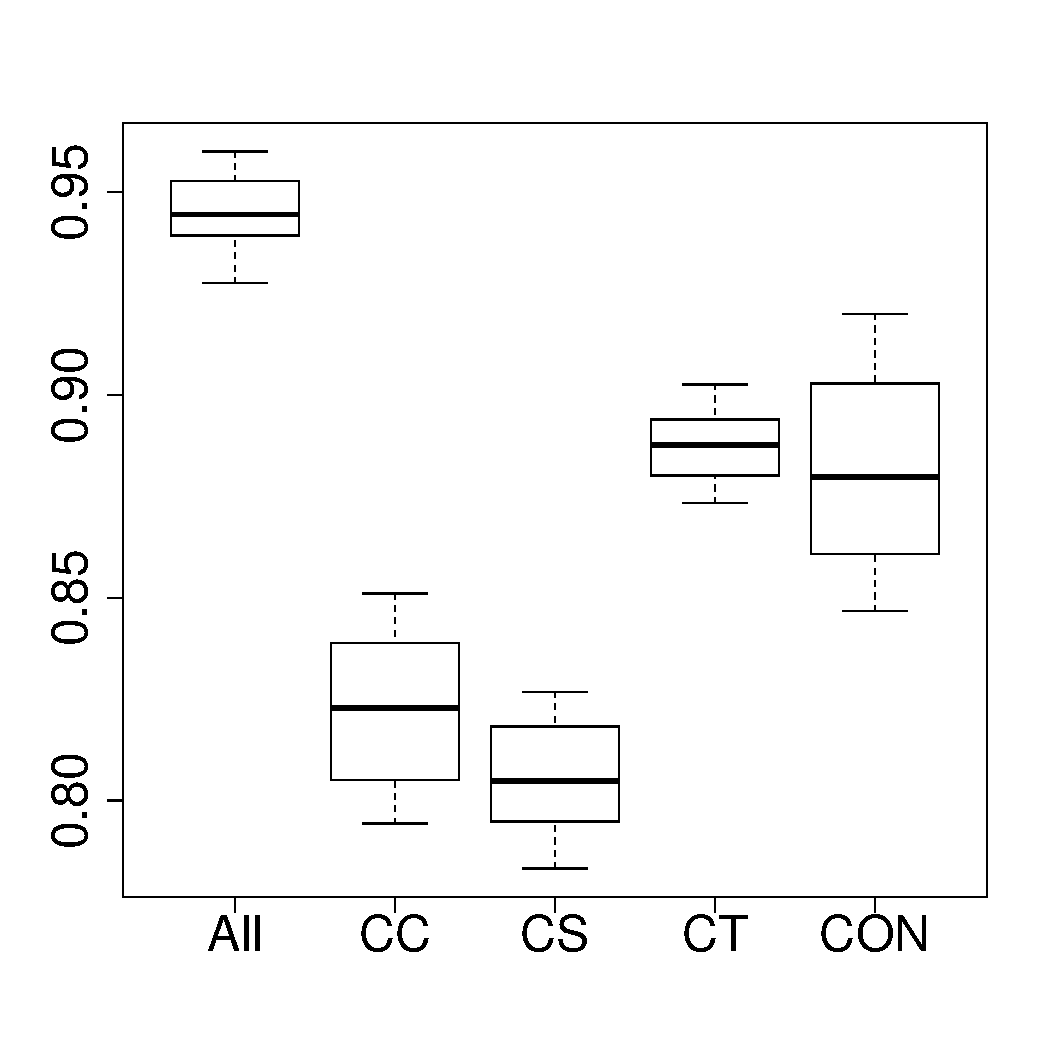
\includegraphics[width=\linewidth]{Figures/runtime-hadoopkeep-importance.pdf}
                \caption{Res. time}
        \end{subfigure}%
        \begin{subfigure}{0.19\textwidth}
                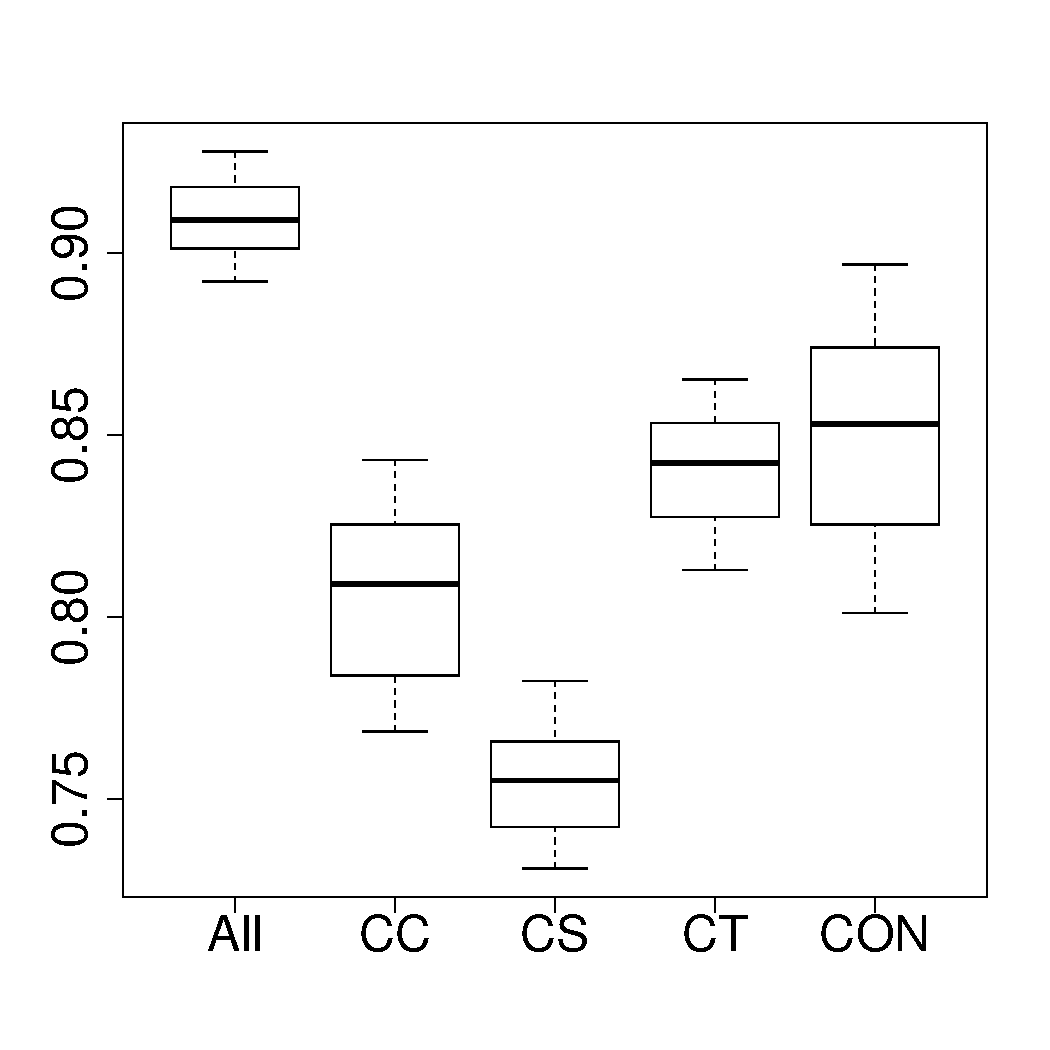
\includegraphics[width=\linewidth]{Figures/cpu-hadoopkeep-importance.pdf}
                \caption{CPU}
        \end{subfigure}%
        \begin{subfigure}{0.19\textwidth}
                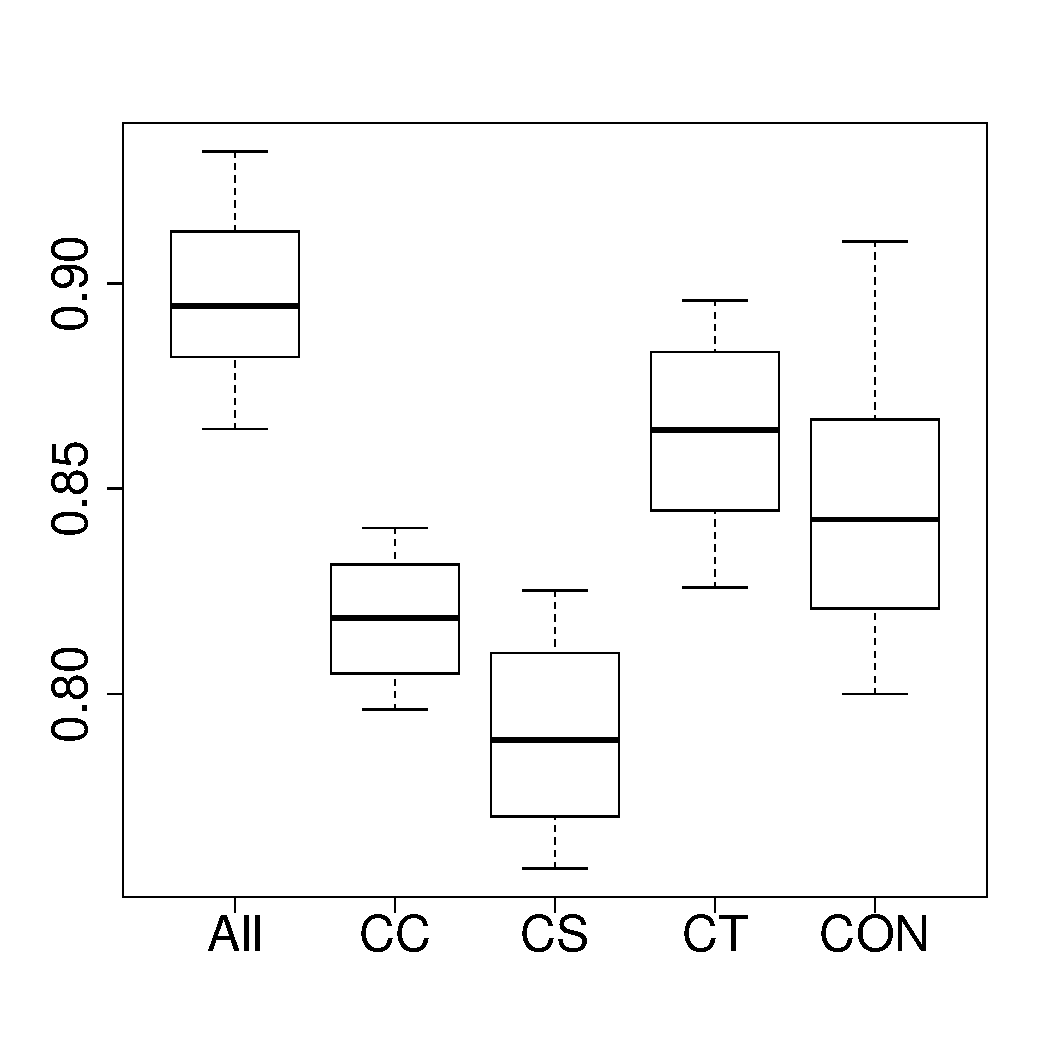
\includegraphics[width=\linewidth]{Figures/mem-hadoopkeep-importance.pdf}
                \caption{Memory}
        \end{subfigure}%
        \begin{subfigure}{0.19\textwidth}
                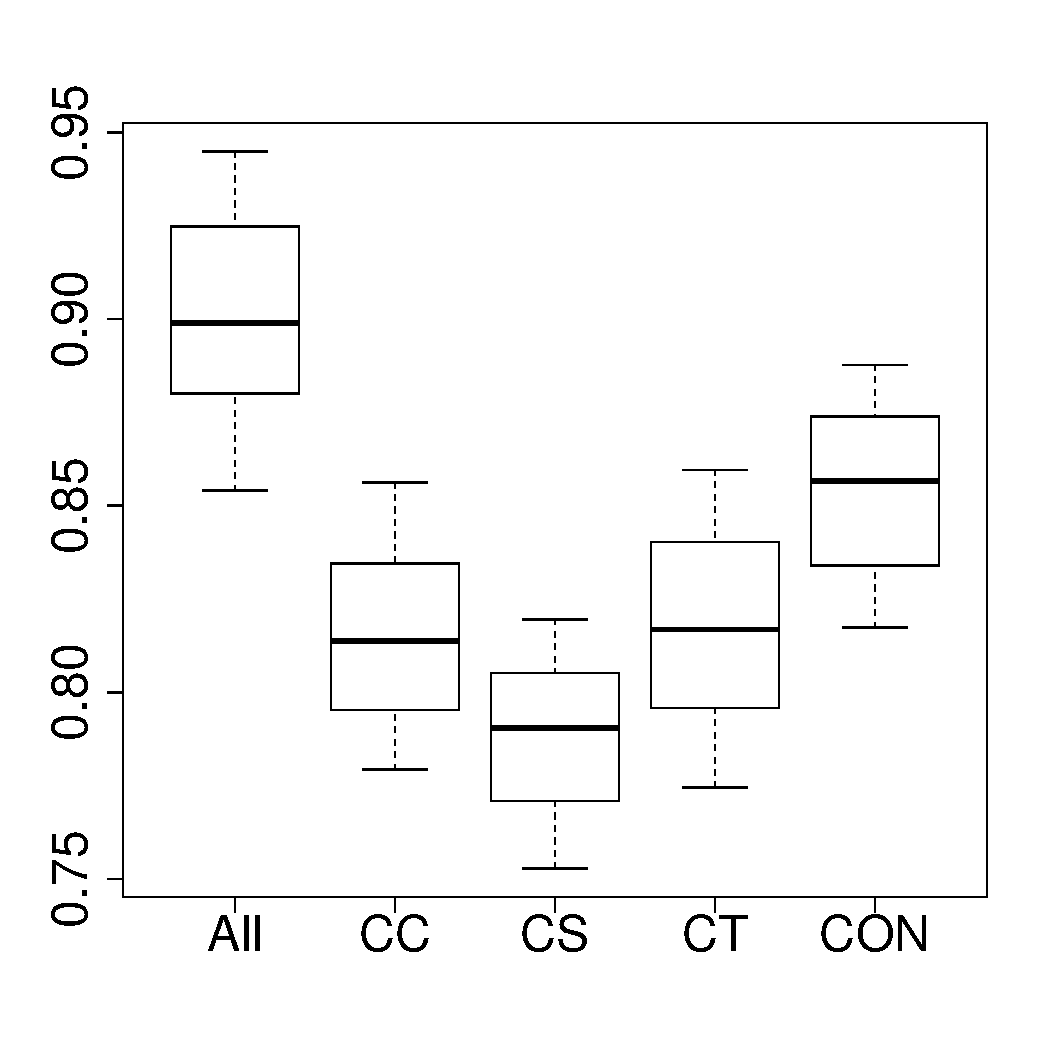
\includegraphics[width=\linewidth]{Figures/ioread-hadoopkeep-importance.pdf}
                \caption{I/O read}
        \end{subfigure}
        \begin{subfigure}{0.19\textwidth}
                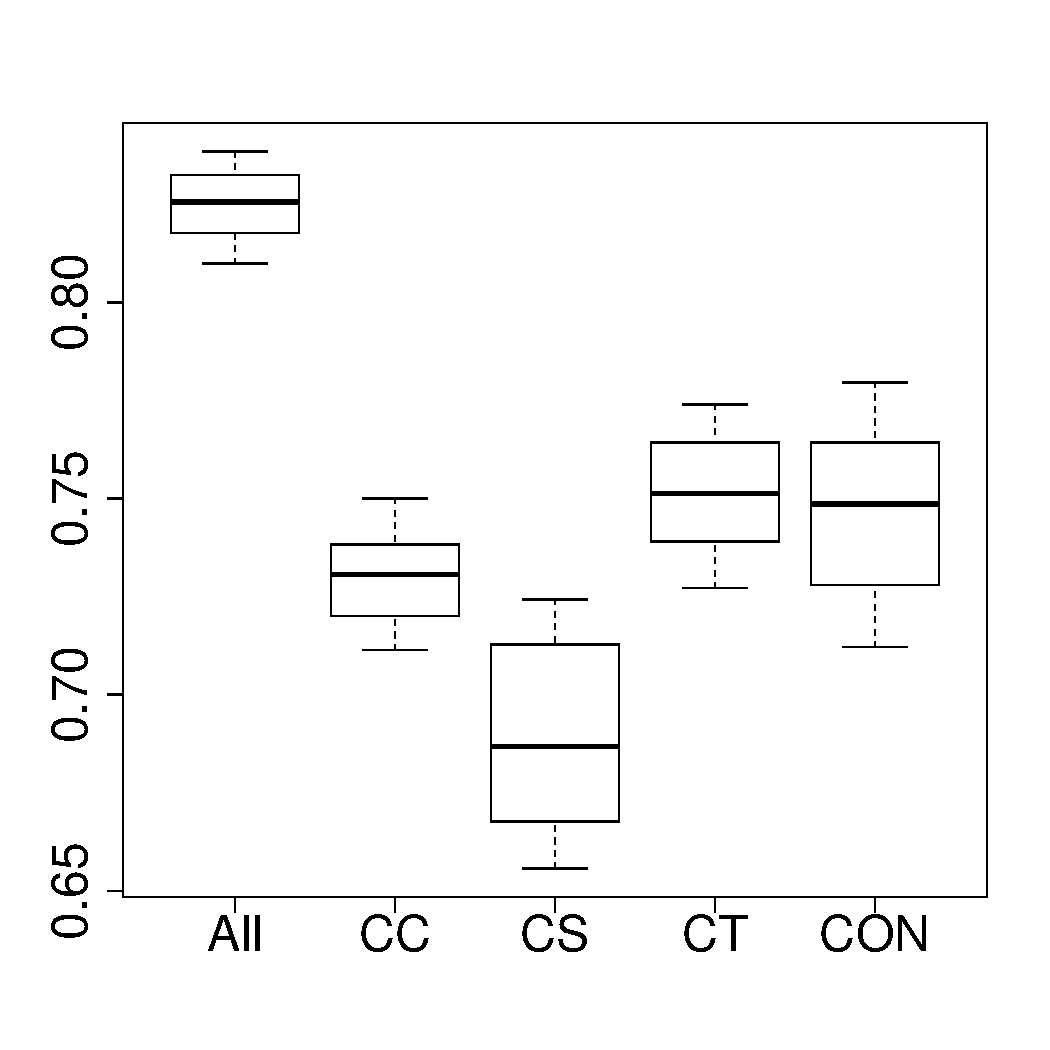
\includegraphics[width=\linewidth]{Figures/iowrite-hadoopkeep-importance.pdf}
                \caption{I/O write}
        \end{subfigure}
        
	\caption{AUC of RF for \emph{Hadoop} when only keeping one dimension of metrics.}
	\label{fig:importance-dimenssion-keep-hadoop}
\end{figure*}

\begin{figure*}[t]
	\centering
        \begin{subfigure}{0.19\textwidth}
                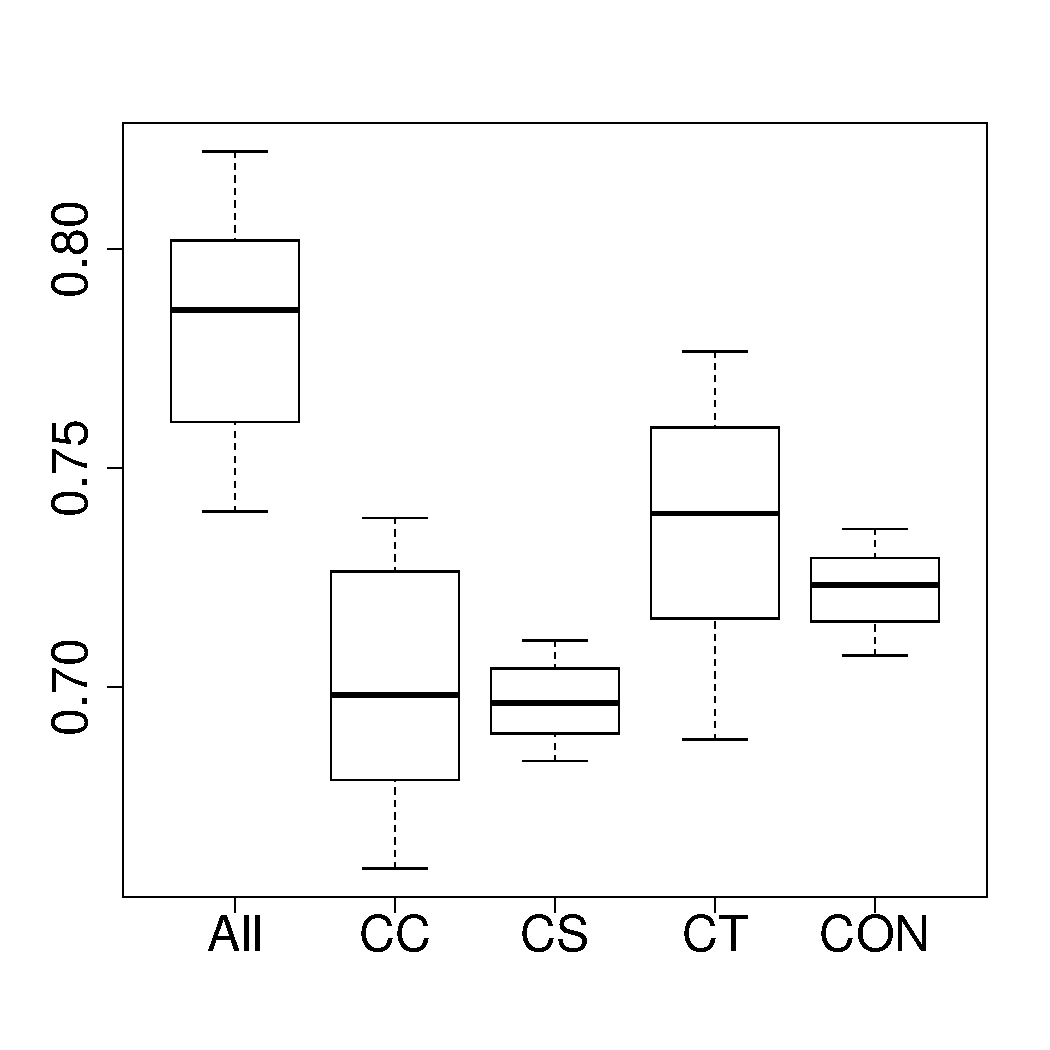
\includegraphics[width=\linewidth]{Figures/runtime-cassandrakeep-importance.pdf}
                \caption{Res. time}
        \end{subfigure}%
        \begin{subfigure}{0.19\textwidth}
                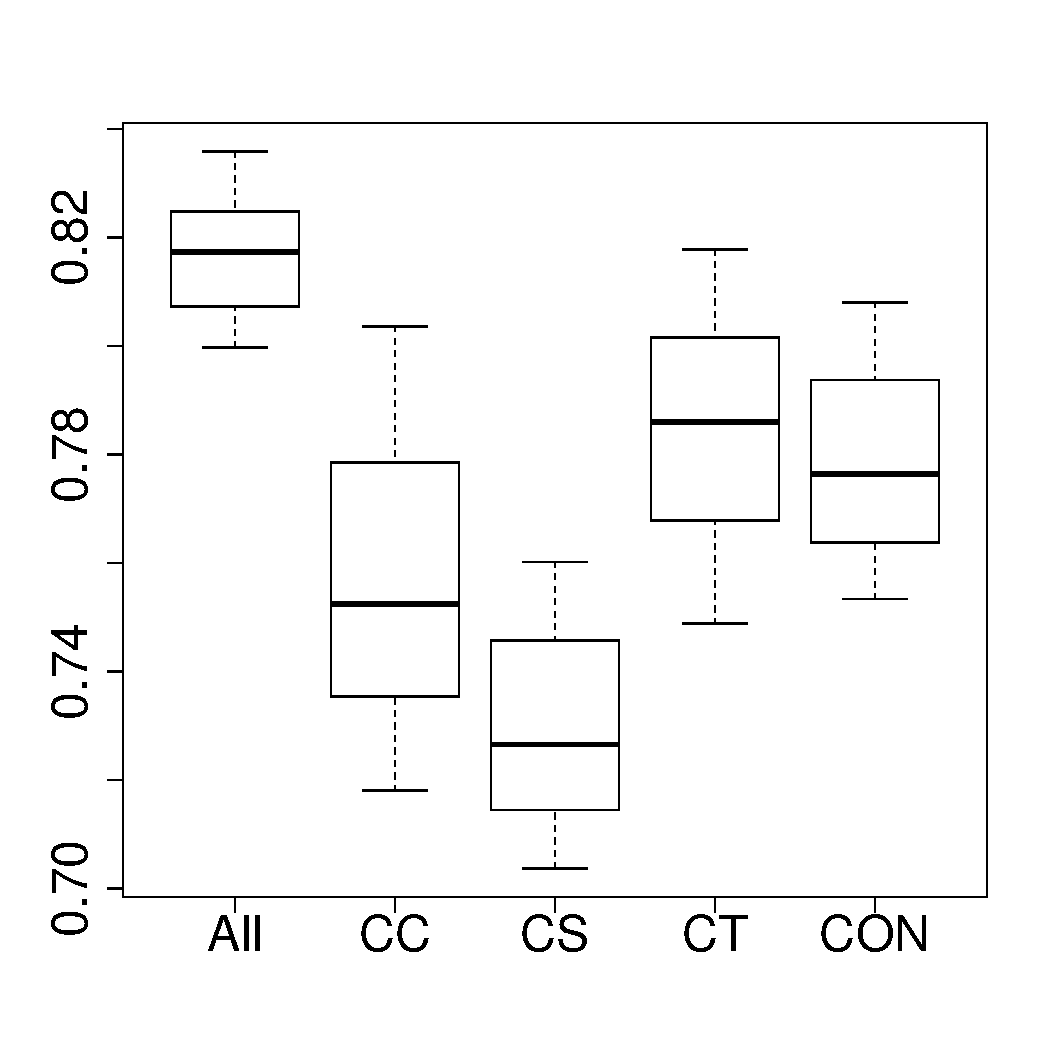
\includegraphics[width=\linewidth]{Figures/cpu-cassandrakeep-importance.pdf}
                \caption{CPU}
        \end{subfigure}%
        \begin{subfigure}{0.19\textwidth}
                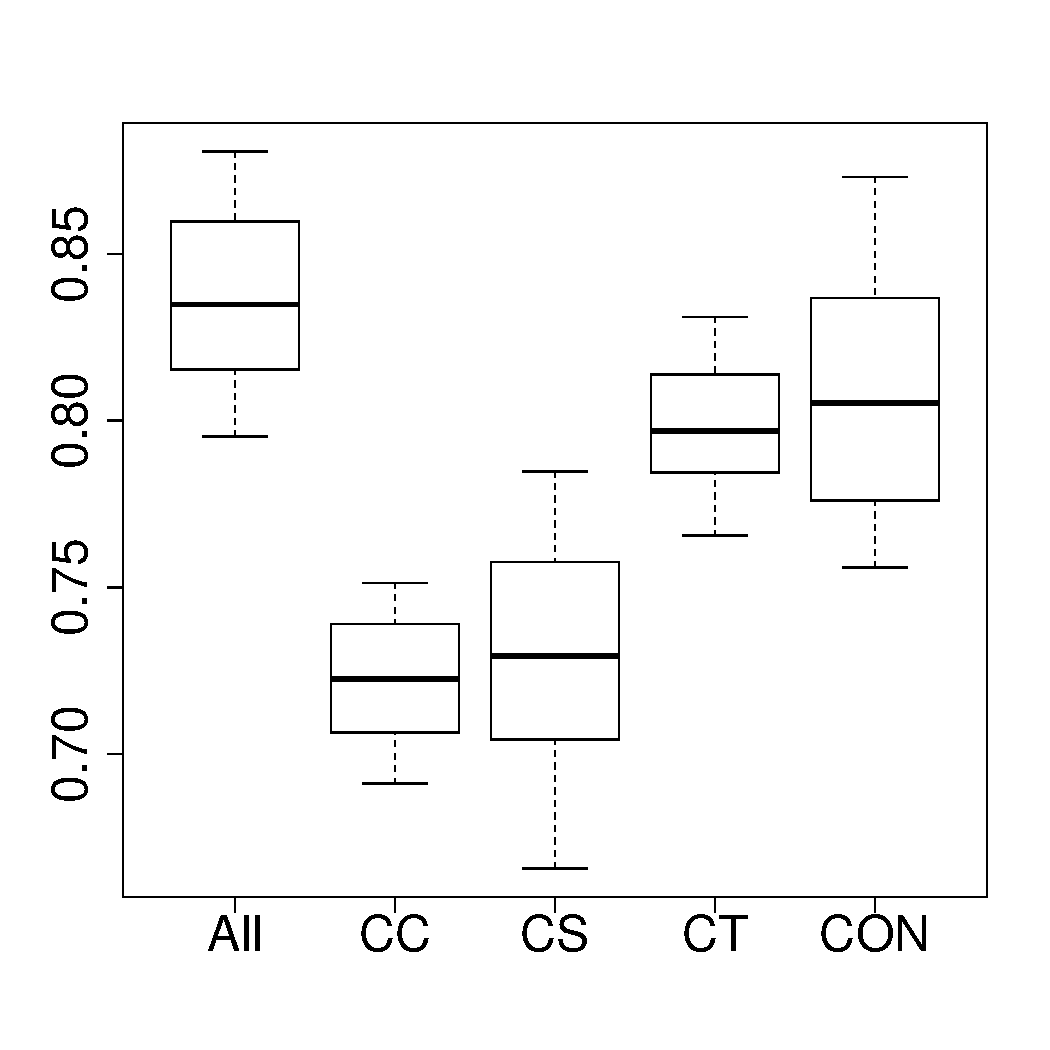
\includegraphics[width=\linewidth]{Figures/mem-cassandrakeep-importance.pdf}
                \caption{Memory}
        \end{subfigure}%
        \begin{subfigure}{0.19\textwidth}
                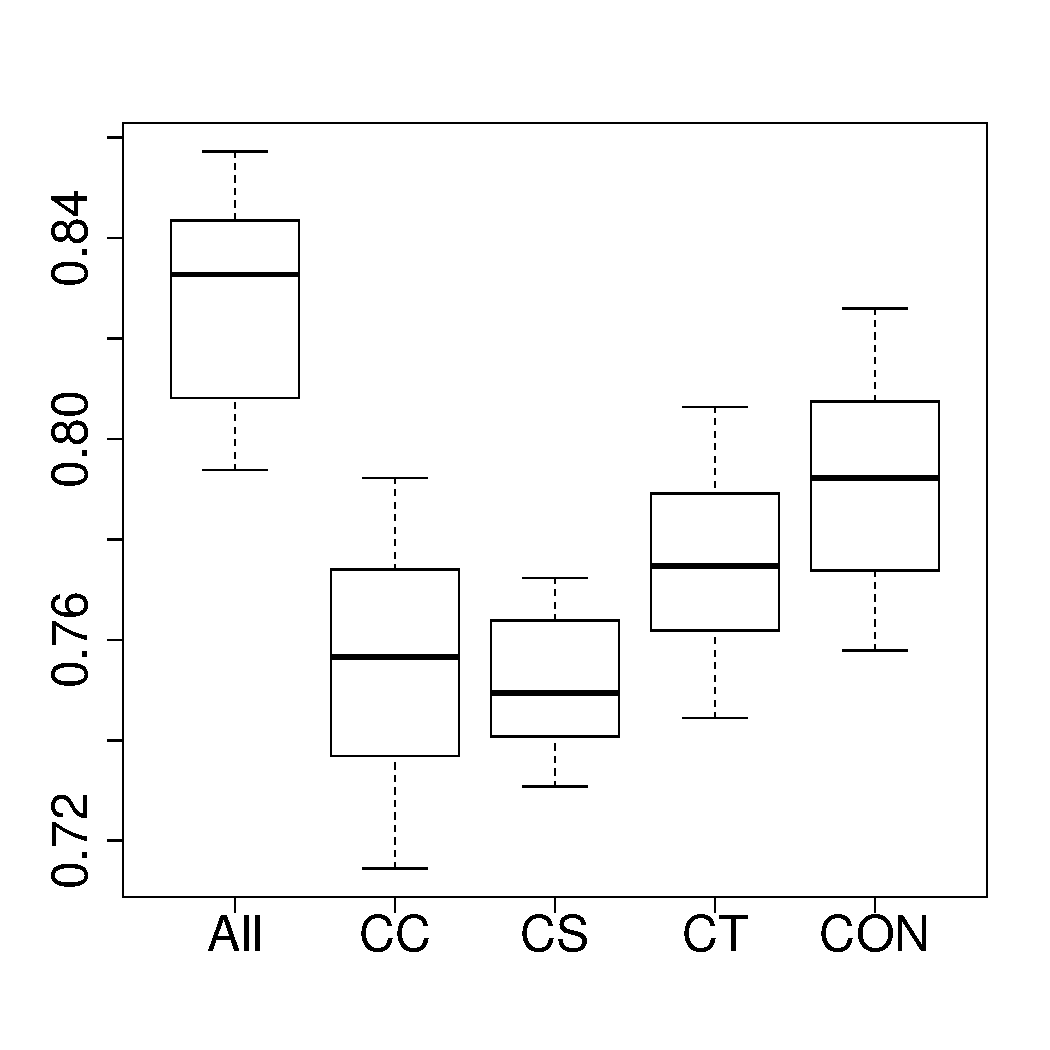
\includegraphics[width=\linewidth]{Figures/ioread-cassandrakeep-importance.pdf}
                \caption{I/O read}
        \end{subfigure}
        \begin{subfigure}{0.19\textwidth}
                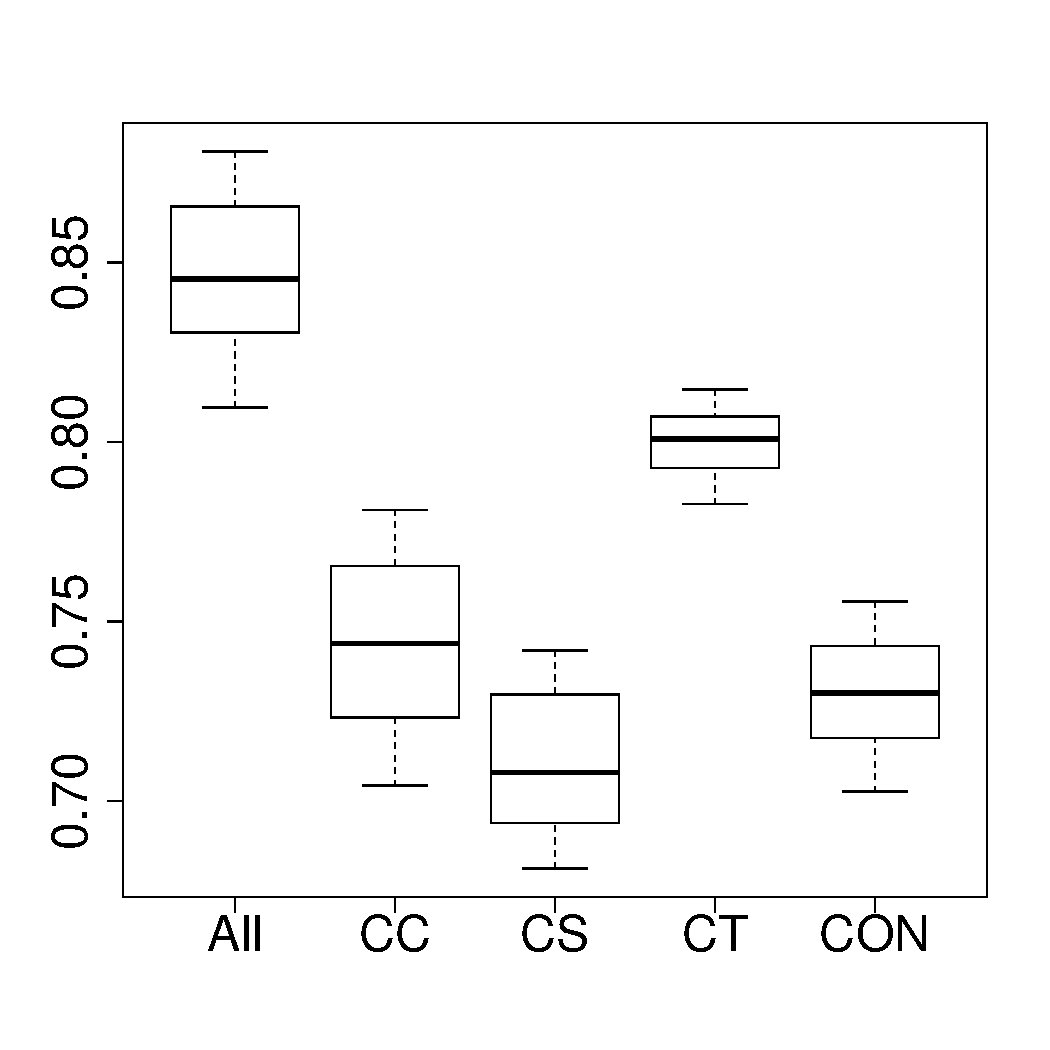
\includegraphics[width=\linewidth]{Figures/iowrite-cassandrakeep-importance.pdf}
                \caption{I/O write}
        \end{subfigure}
        
	\caption{AUC of RF for \emph{Cassandra} when only keeping one dimension of metrics.}
	\label{fig:importance-dimenssion-keep-cassandra}
\end{figure*}

\begin{figure*}[t]
	\centering
        \begin{subfigure}{0.19\textwidth}
                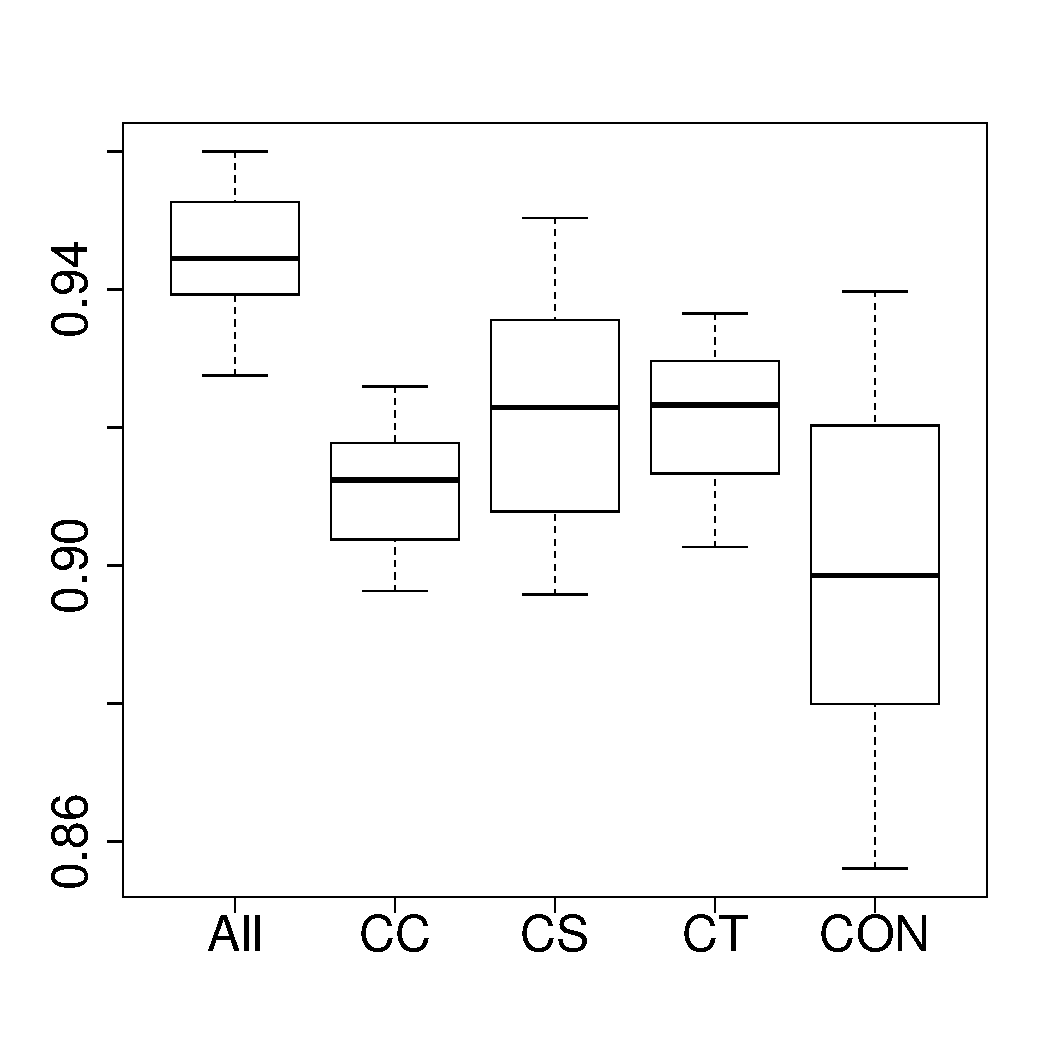
\includegraphics[width=\linewidth]{Figures/runtime-hadoopremove-importance.pdf}
                \caption{Res. time}
        \end{subfigure}%
        \begin{subfigure}{0.19\textwidth}
                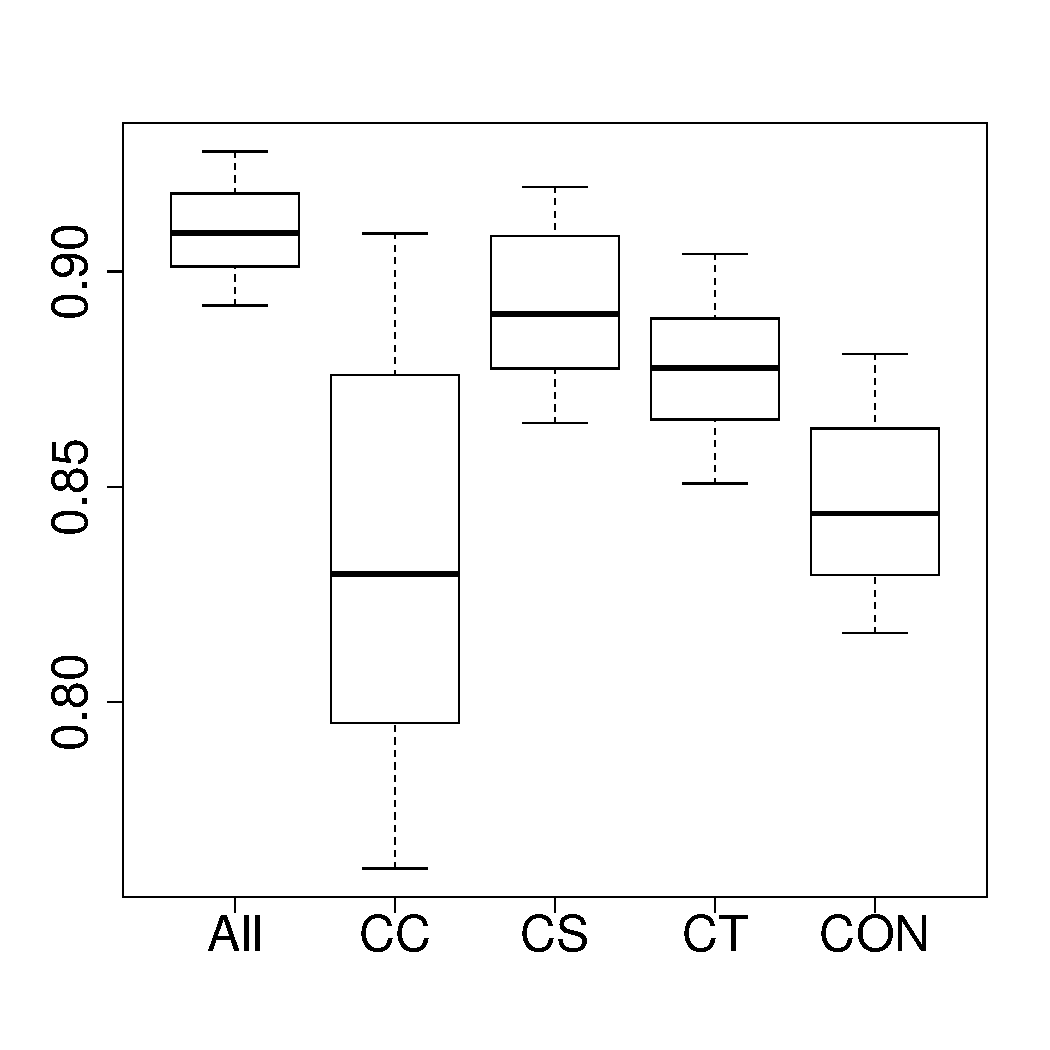
\includegraphics[width=\linewidth]{Figures/cpu-hadoopremove-importance.pdf}
                \caption{CPU}
        \end{subfigure}%
        \begin{subfigure}{0.19\textwidth}
                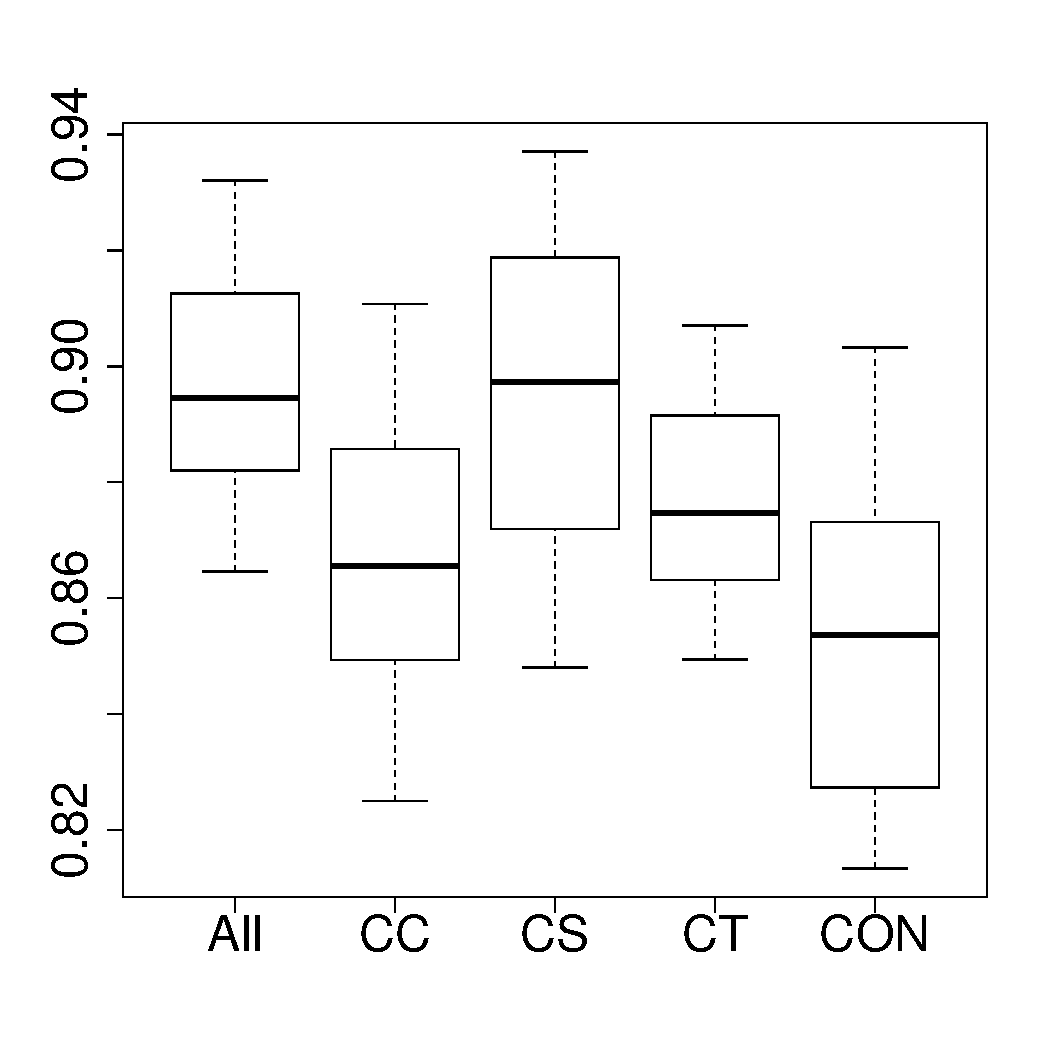
\includegraphics[width=\linewidth]{Figures/mem-hadoopremove-importance.pdf}
                \caption{Memory}
        \end{subfigure}%
        \begin{subfigure}{0.19\textwidth}
                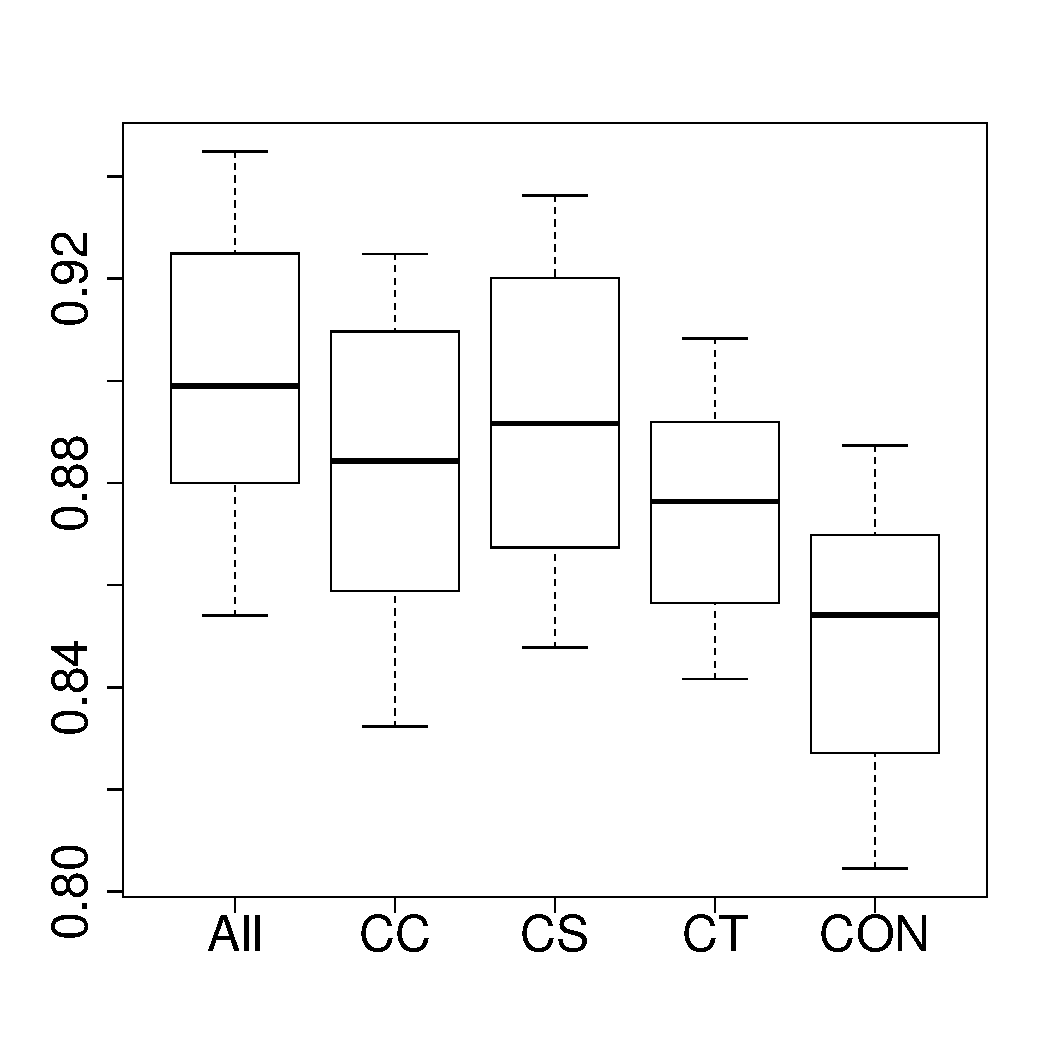
\includegraphics[width=\linewidth]{Figures/ioread-hadoopremove-importance.pdf}
                \caption{I/O read}
        \end{subfigure}
        \begin{subfigure}{0.19\textwidth}
                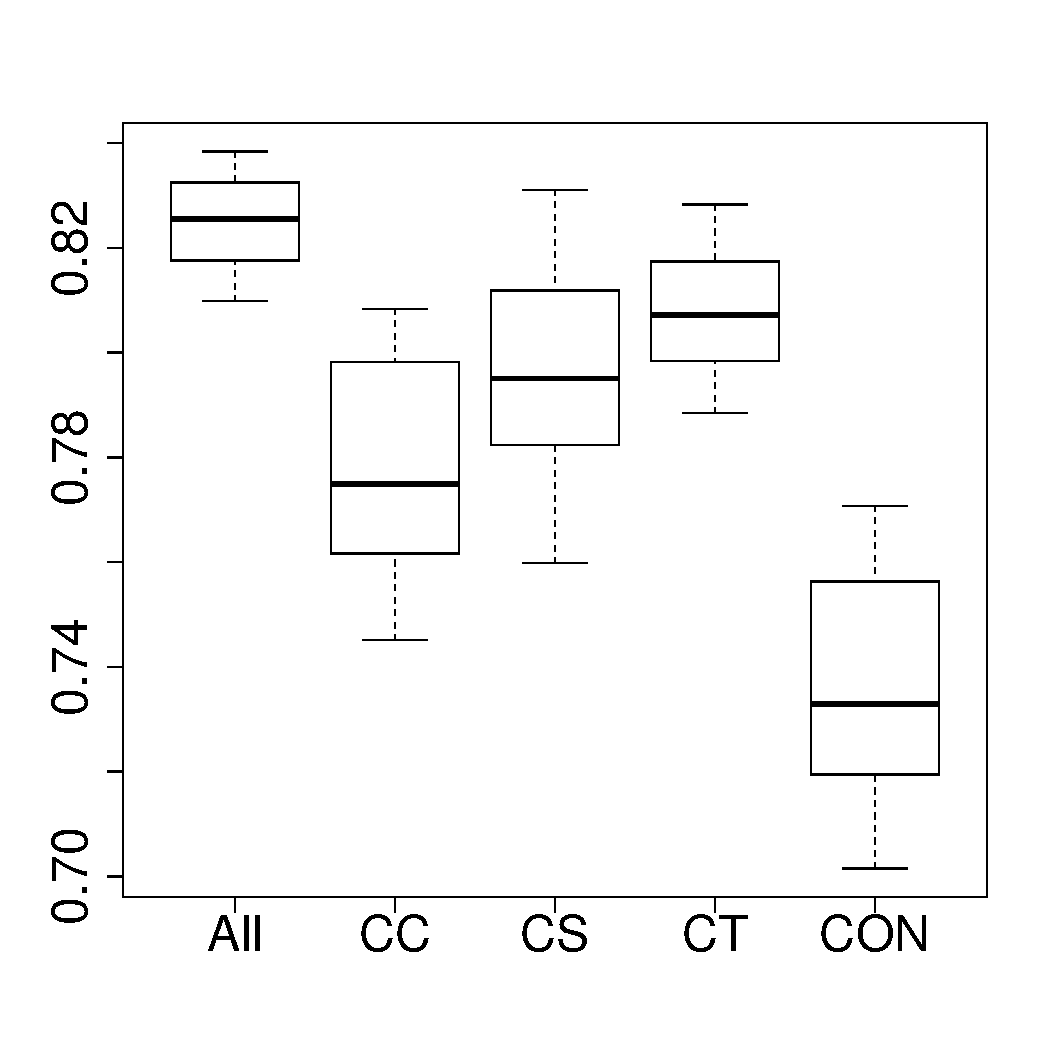
\includegraphics[width=\linewidth]{Figures/iowrite-hadoopremove-importance.pdf}
                \caption{I/O write}
        \end{subfigure}
        
	\caption{AUC of RF for \emph{Hadoop} when removing one dimension of metrics.}
	\label{fig:importance-dimenssion-remove-hadoop}
\end{figure*}

\begin{figure*}[t]
	\centering
        \begin{subfigure}{0.19\textwidth}
                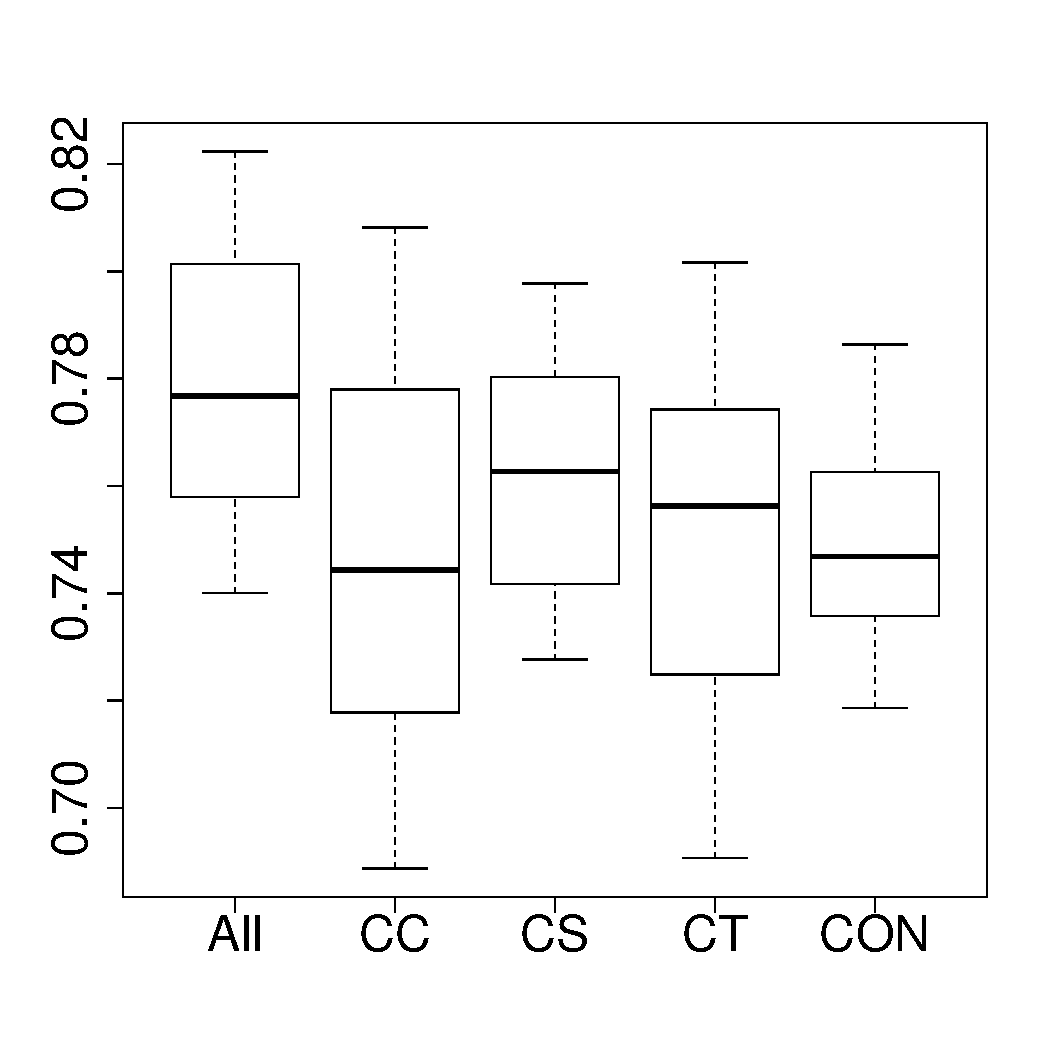
\includegraphics[width=\linewidth]{Figures/runtime-cassandraremove-importance.pdf}
                \caption{Res. time}
        \end{subfigure}%
        \begin{subfigure}{0.19\textwidth}
                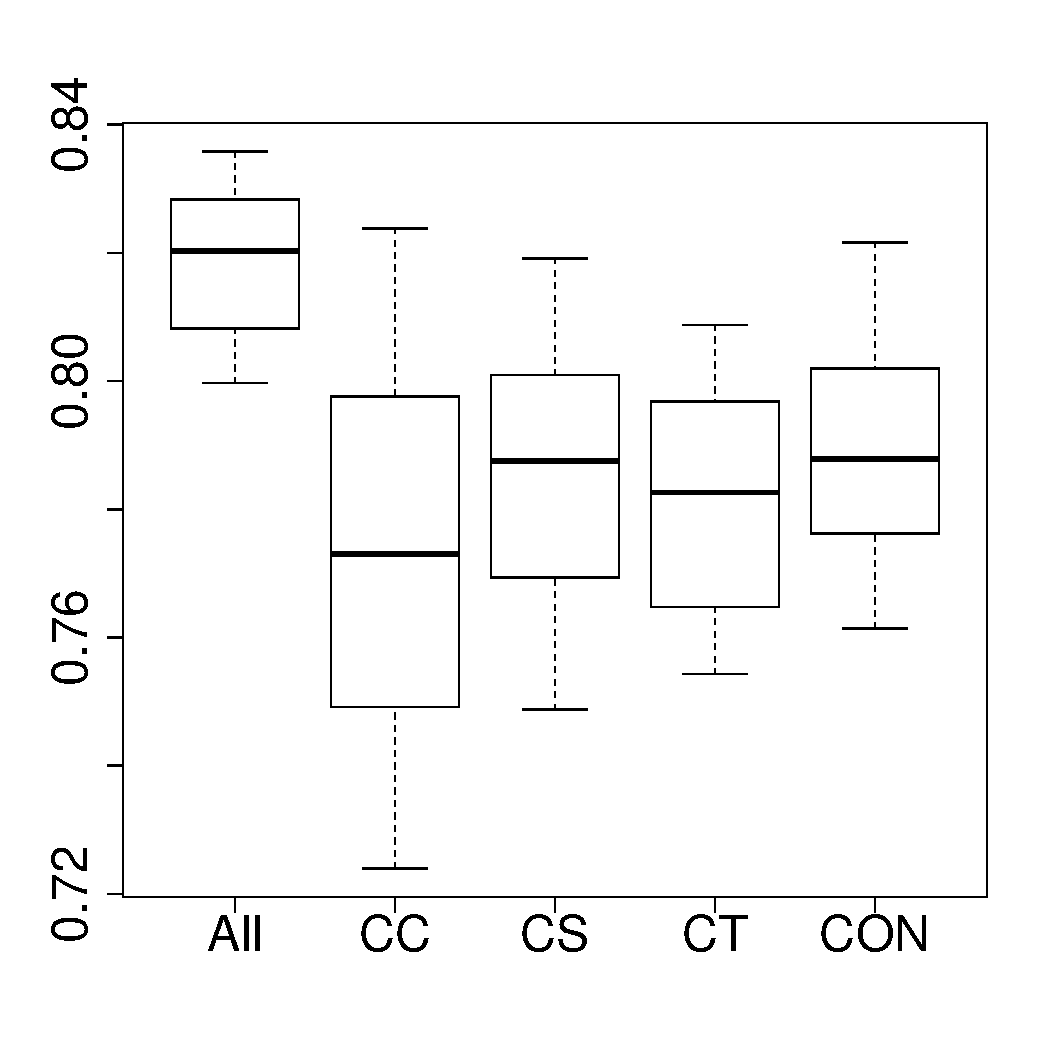
\includegraphics[width=\linewidth]{Figures/cpu-cassandraremove-importance.pdf}
                \caption{CPU}
        \end{subfigure}%
        \begin{subfigure}{0.19\textwidth}
                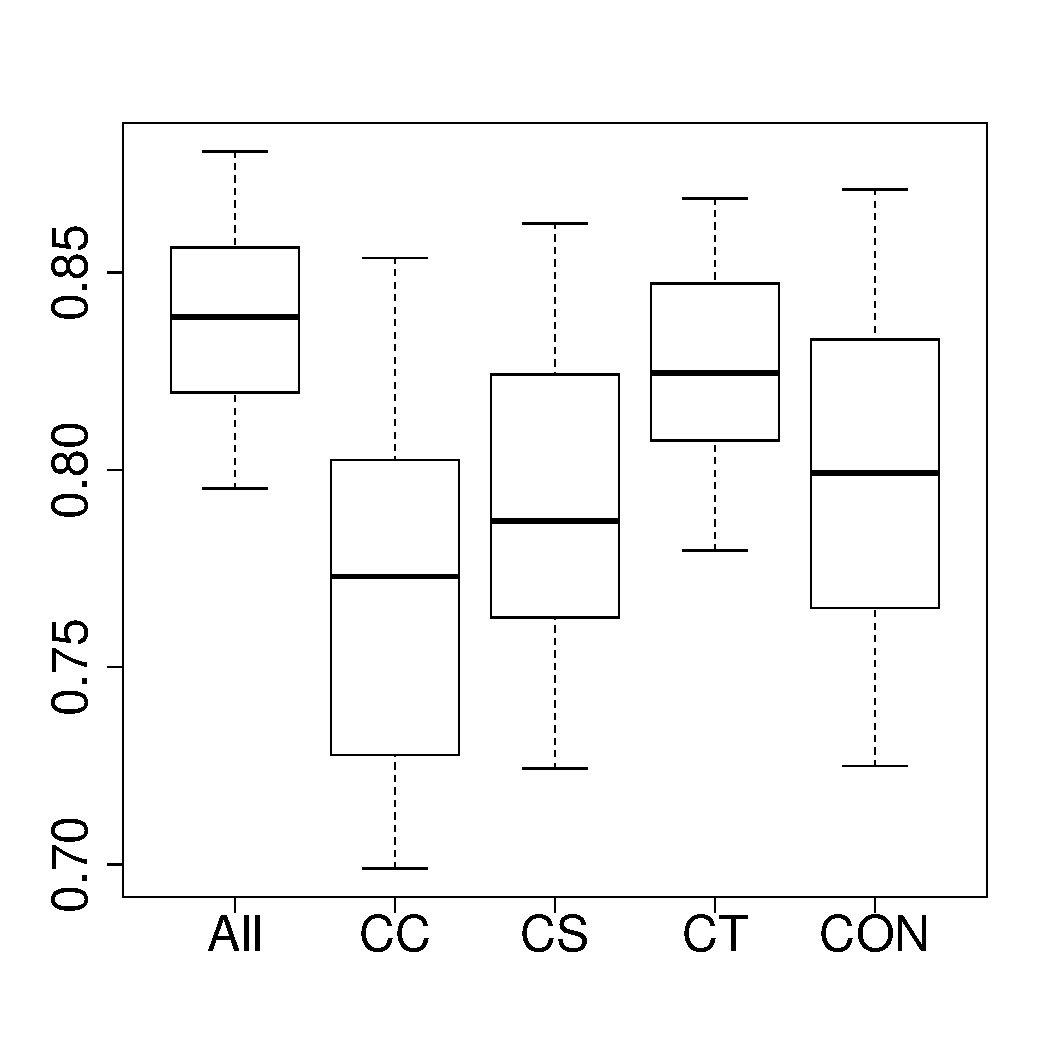
\includegraphics[width=\linewidth]{Figures/mem-cassandraremove-importance.pdf}
                \caption{Memory}
        \end{subfigure}%
        \begin{subfigure}{0.19\textwidth}
                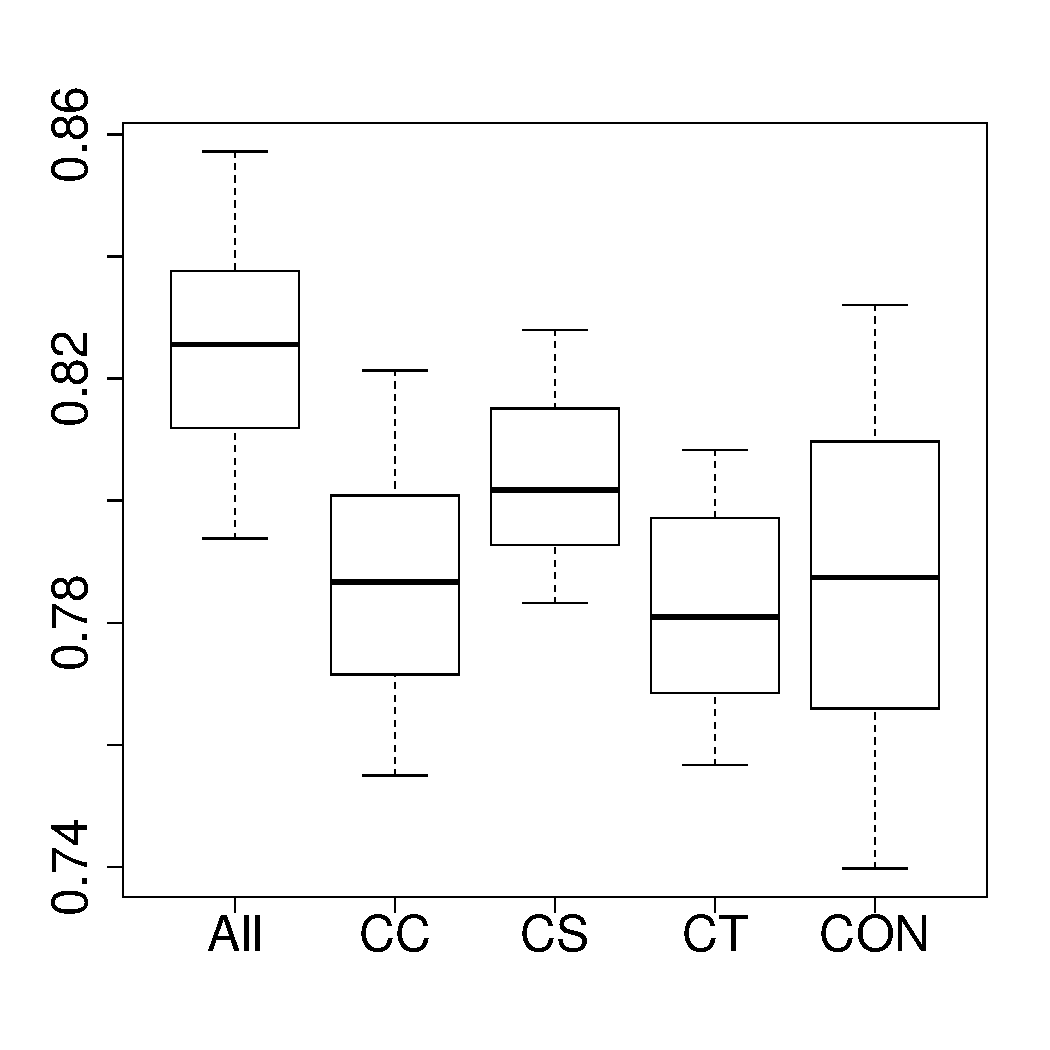
\includegraphics[width=\linewidth]{Figures/ioread-cassandraremove-importance.pdf}
                \caption{I/O read}
        \end{subfigure}
        \begin{subfigure}{0.19\textwidth}
                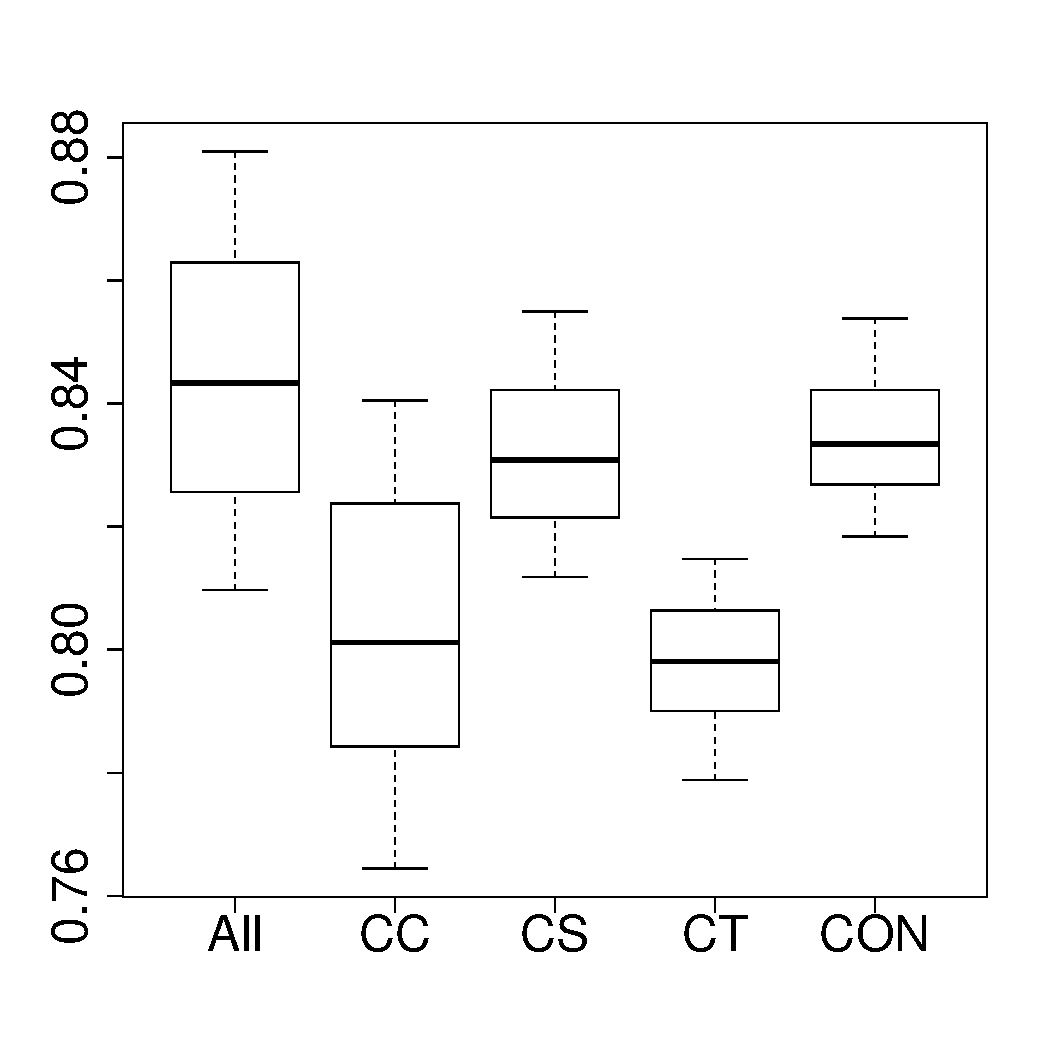
\includegraphics[width=\linewidth]{Figures/iowrite-cassandraremove-importance.pdf}
                \caption{I/O write}
        \end{subfigure}
        
	\caption{AUC of RF for \emph{Cassandra} when removing one dimension of metrics.} %\heng{the last box-plots have no label.} \heng{Make all the x/y labels bigger}}
	\label{fig:importance-dimenssion-remove-cassandra}
\end{figure*}


\end{document}